\newcommand\invisiblesection[1]{%
  \refstepcounter{section}%
  \addcontentsline{toc}{section}{#1}%
  \sectionmark{#1}}

\refstepcounter{chapter}
\addcontentsline{toc}{chapter}{Full Papers}
\sectionmark{Full Papers}

\invisiblesection{Nataly Jahchan, Anne Condamines, Emmanuelle Cannesson and Helene Giraudo. Towards a More Natural Controlled Language in Future Airbus Cockpits. A Psycho-linguistic Evaluation}
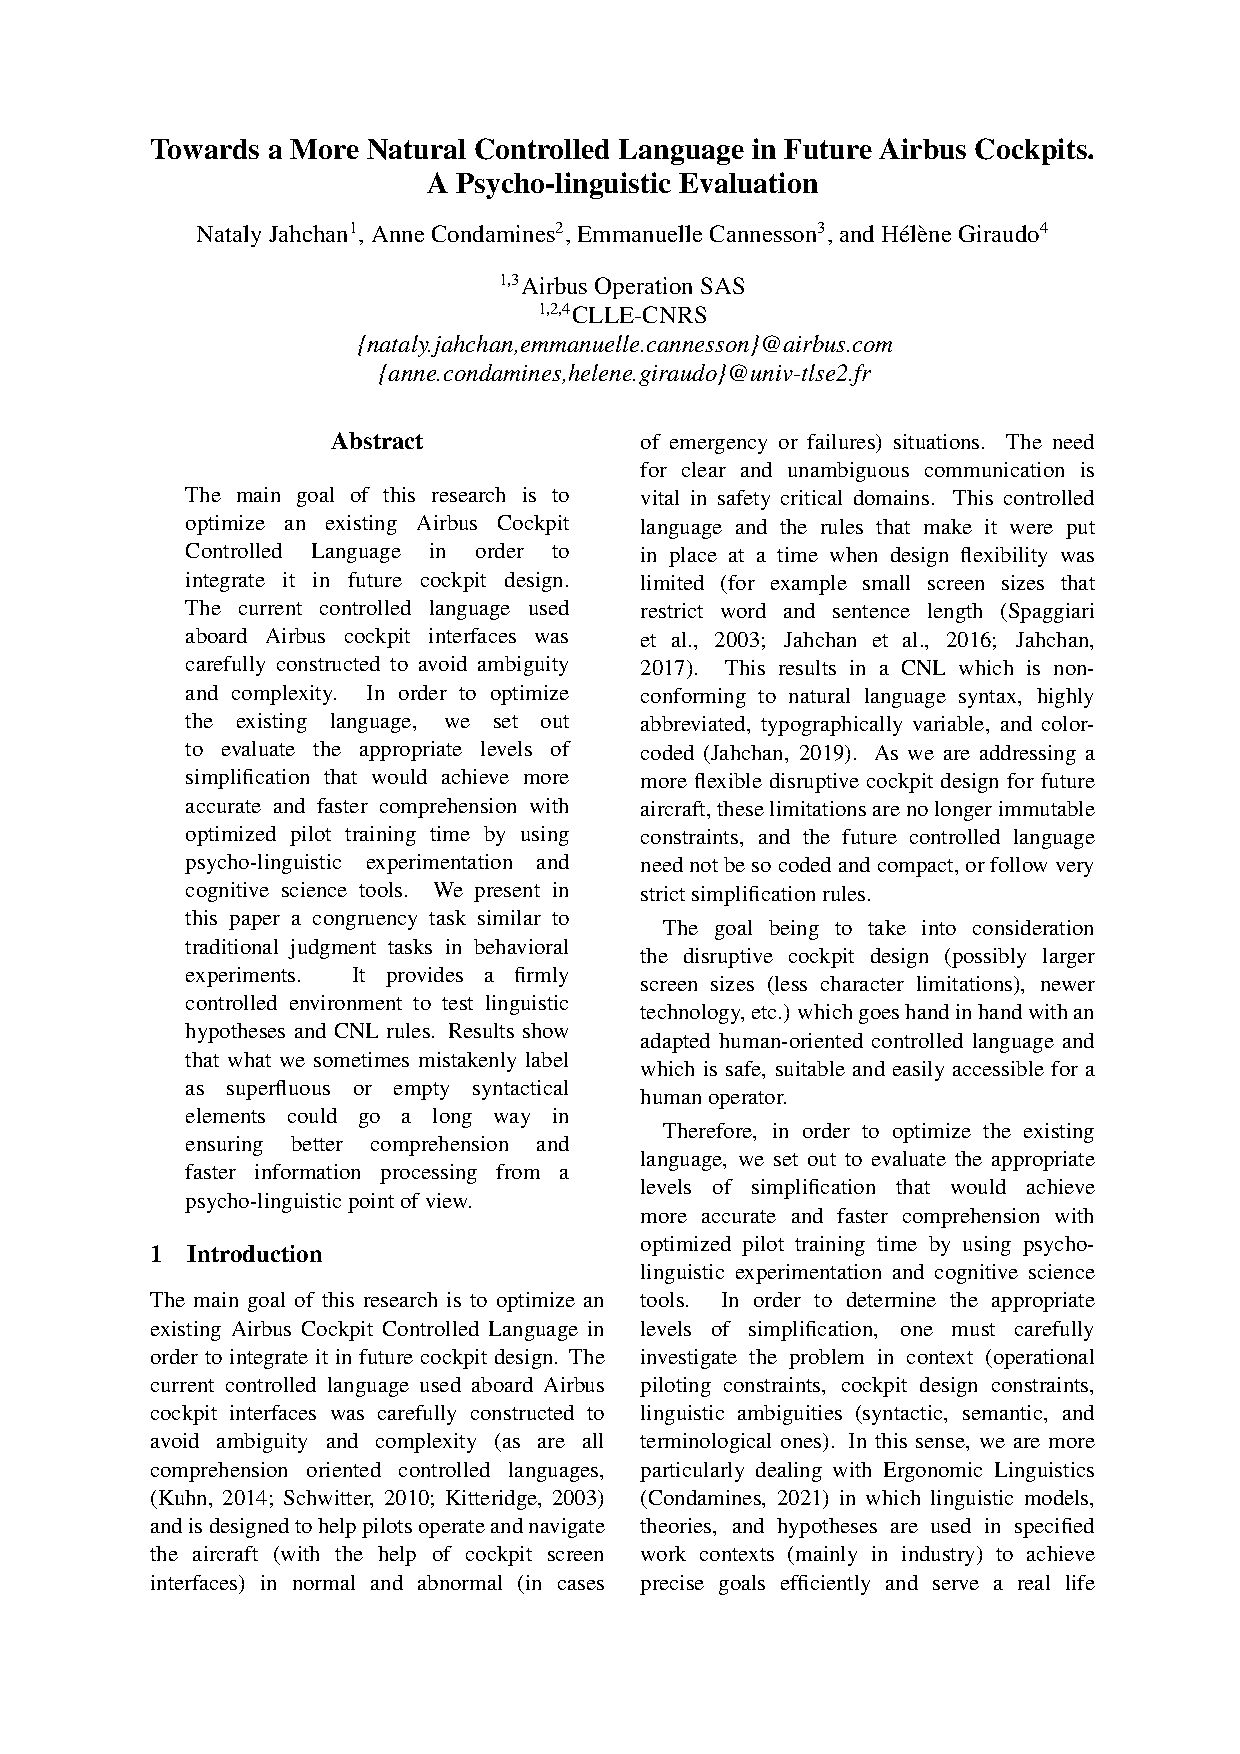
\includepdf[pages=-,pagecommand={}]{../cdrom/pdf/2021.cnl-1.1.pdf}

\invisiblesection{Arianna Masciolini and Aarne Ranta. Grammar-Based Concept Alignment for Domain-Specific Machine Translation}
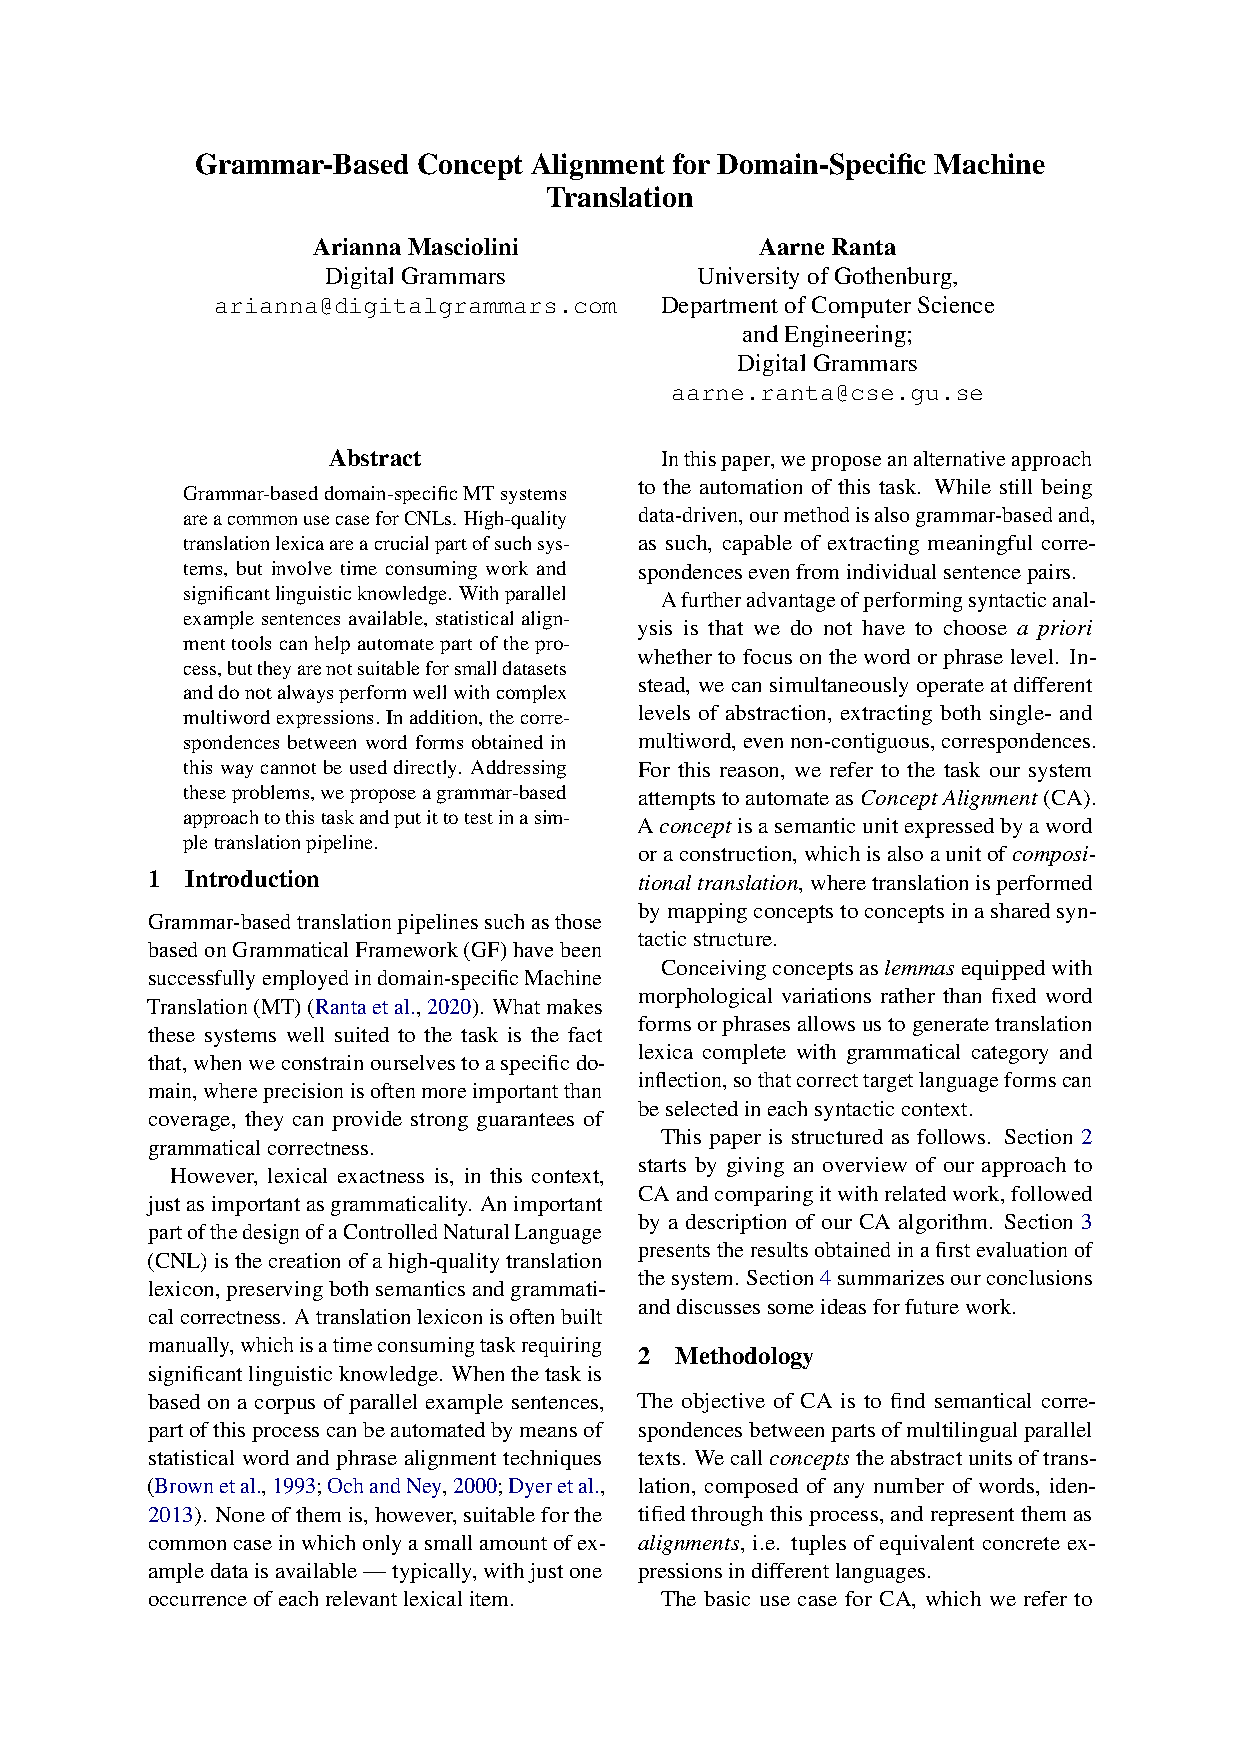
\includepdf[pages=-,pagecommand={}]{../cdrom/pdf/2021.cnl-1.2.pdf}

\invisiblesection{Yannis Haralambous and Tian Tian. Tailoring a Controlled Language Out of a Corpus of Maintenance Reports}
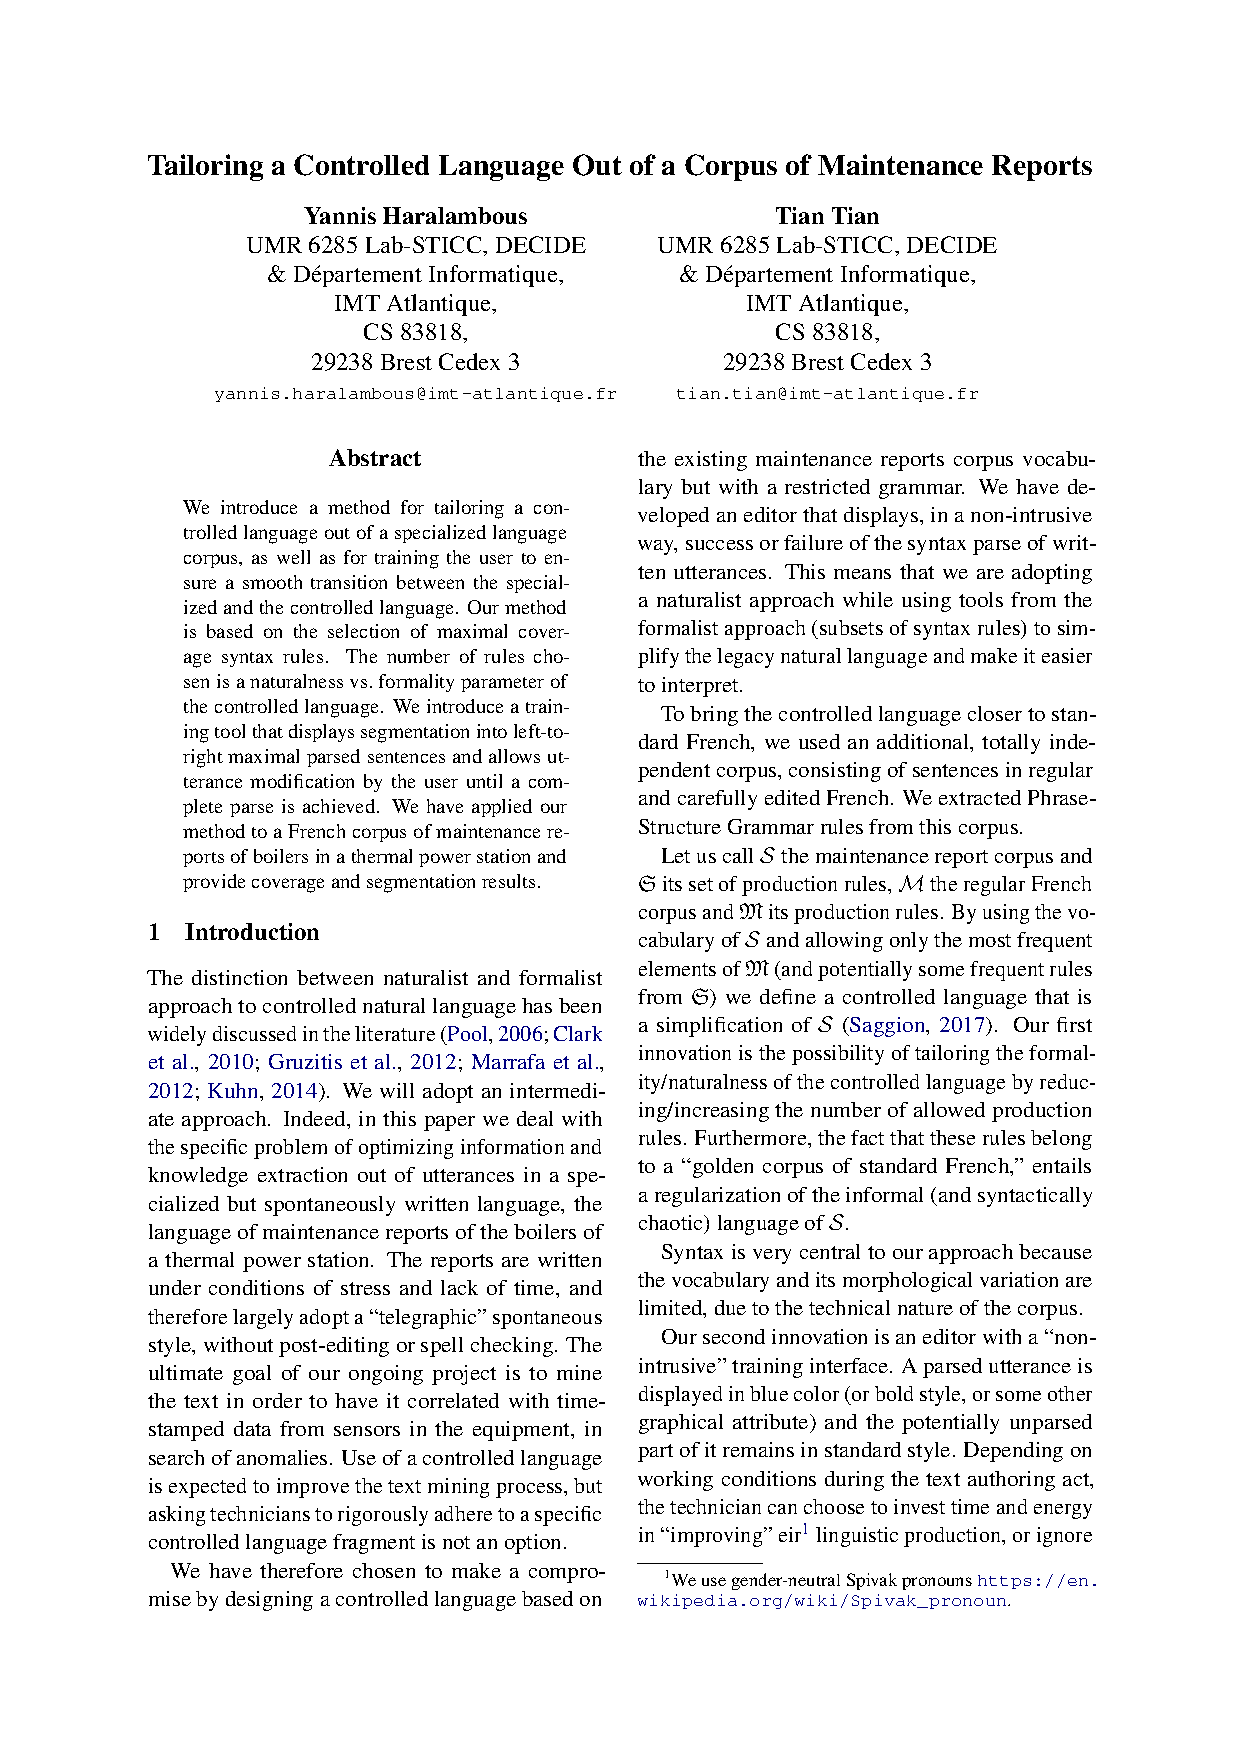
\includepdf[pages=-,pagecommand={}]{../cdrom/pdf/2021.cnl-1.3.pdf}

\invisiblesection{Laurette Marais. Approximating a Zulu GF concrete syntax with a neural network for natural language understanding}
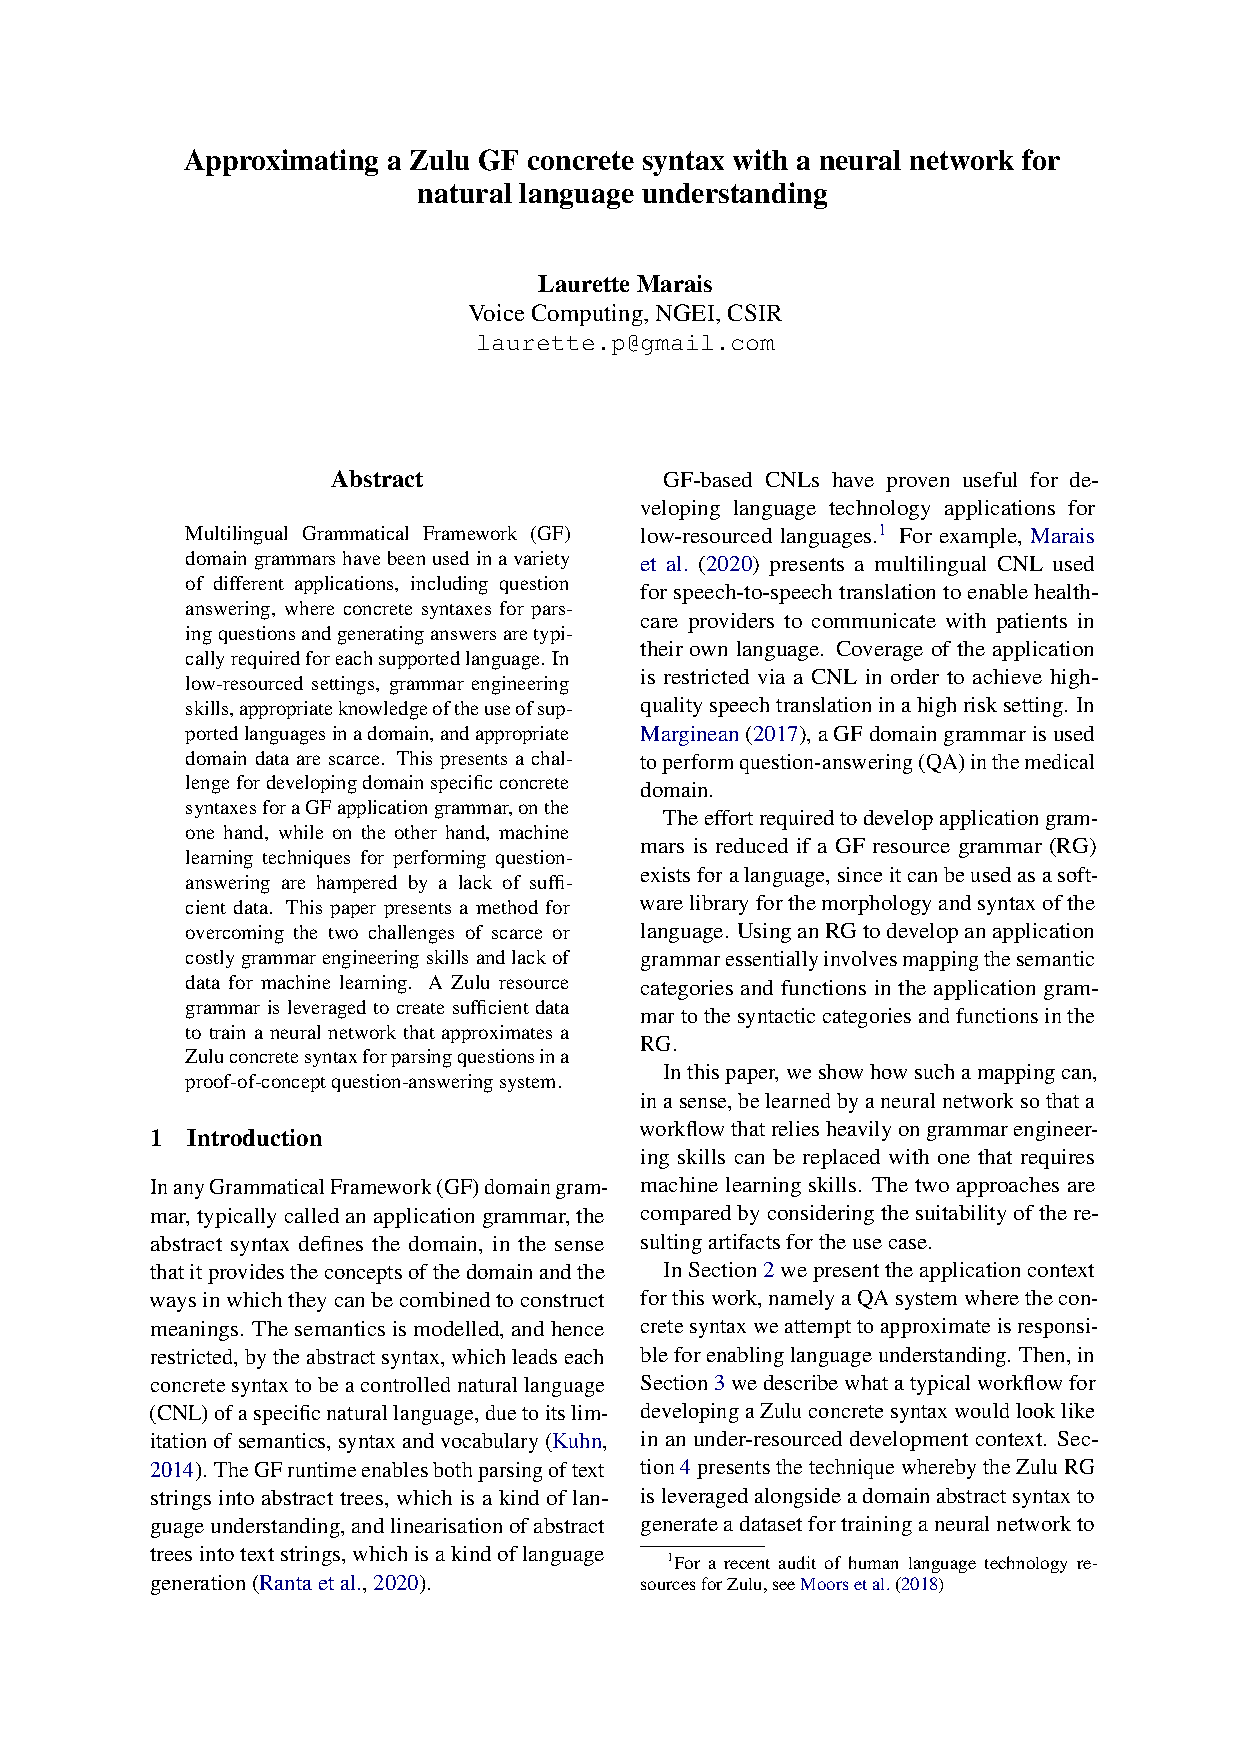
\includepdf[pages=-,pagecommand={}]{../cdrom/pdf/2021.cnl-1.4.pdf}

\invisiblesection{Rolf Schwitter. The Grammar of PENG ASP Explained}
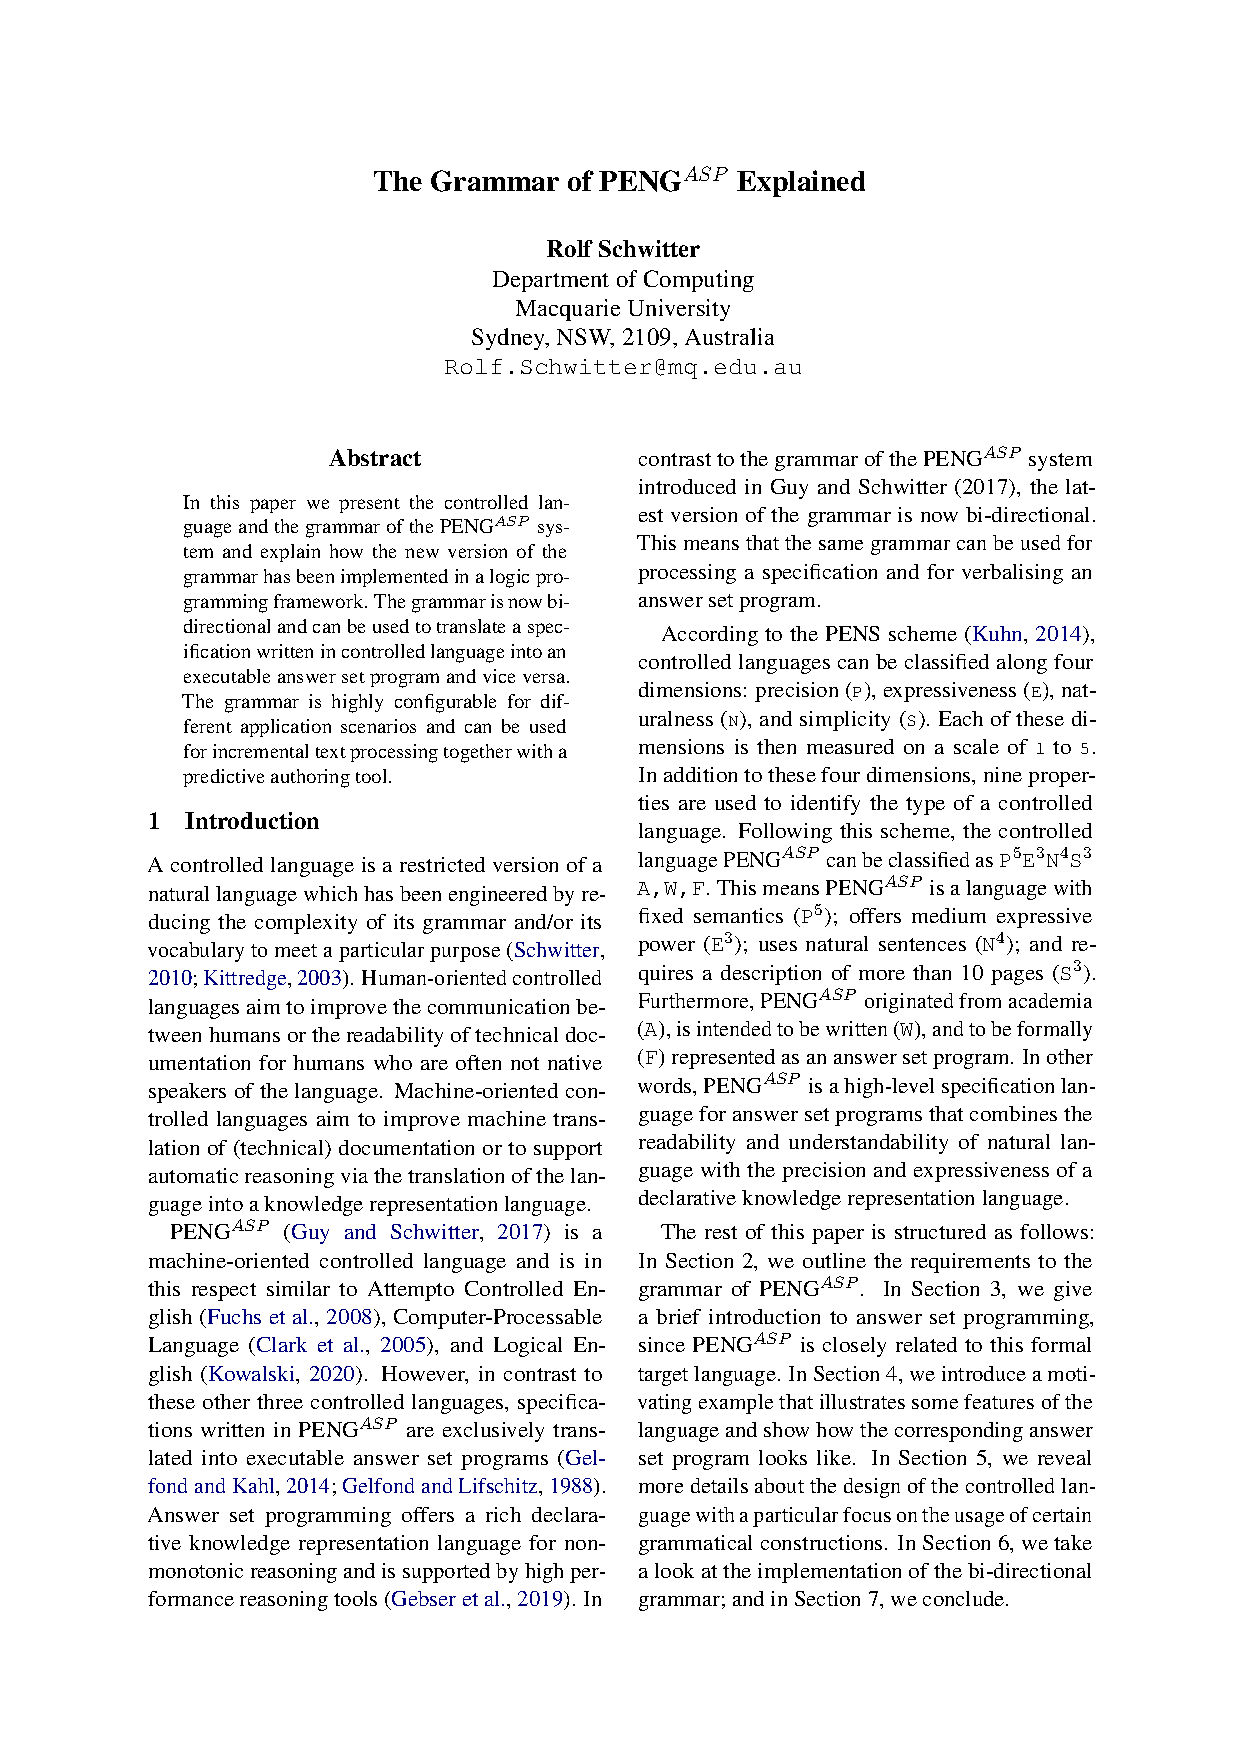
\includepdf[pages=-,pagecommand={}]{../cdrom/pdf/2021.cnl-1.5.pdf}

\invisiblesection{Mischa Corsius, Stijn Hoppenbrouwers, Mariette Lokin, Elian Baars, Gertrude Sangers-Van Cappellen and Ilona Wilmont. RegelSpraak: a CNL for Executable Tax Rules Specification}
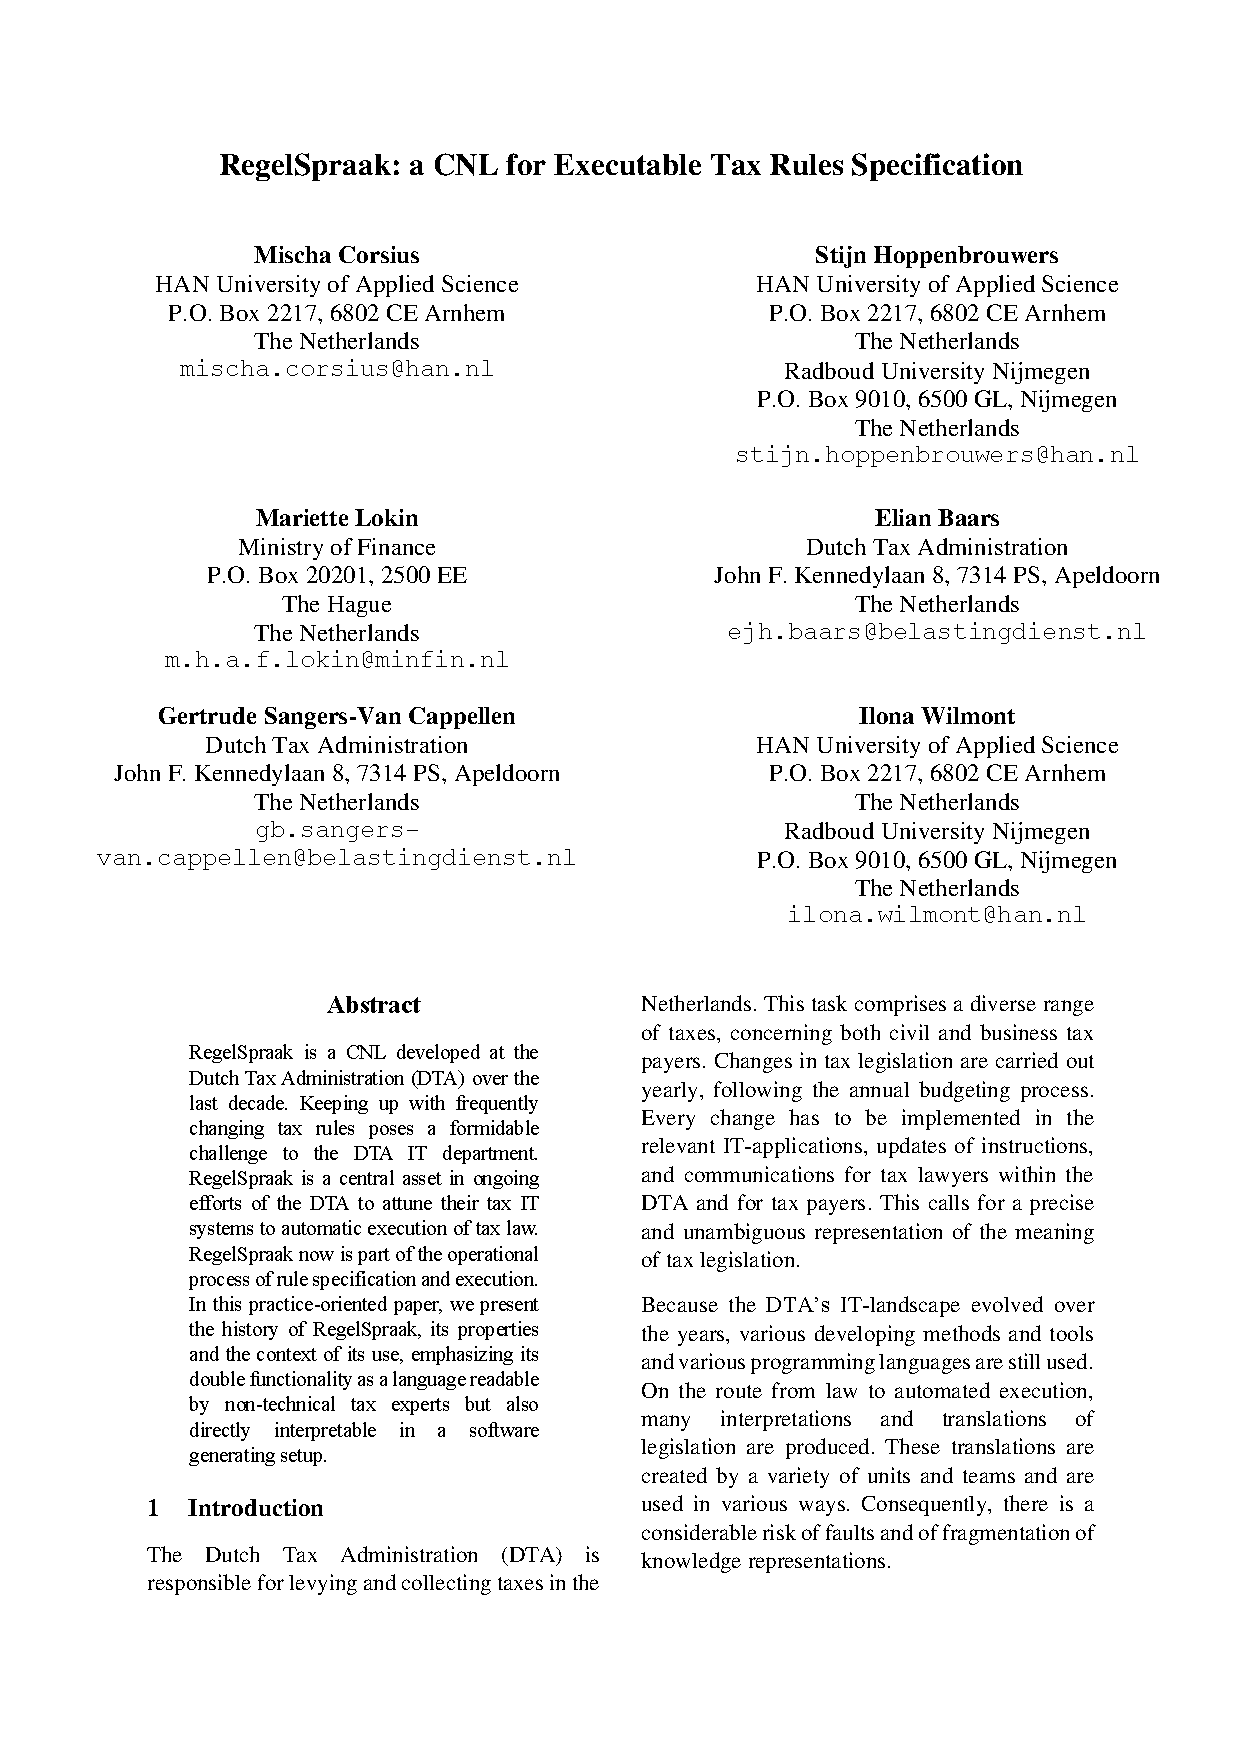
\includepdf[pages=-,pagecommand={}]{../cdrom/pdf/2021.cnl-1.6.pdf}

\invisiblesection{Norbert E. Fuchs. The Law of Inertia and the Frame Problem in Attempto Controlled English}
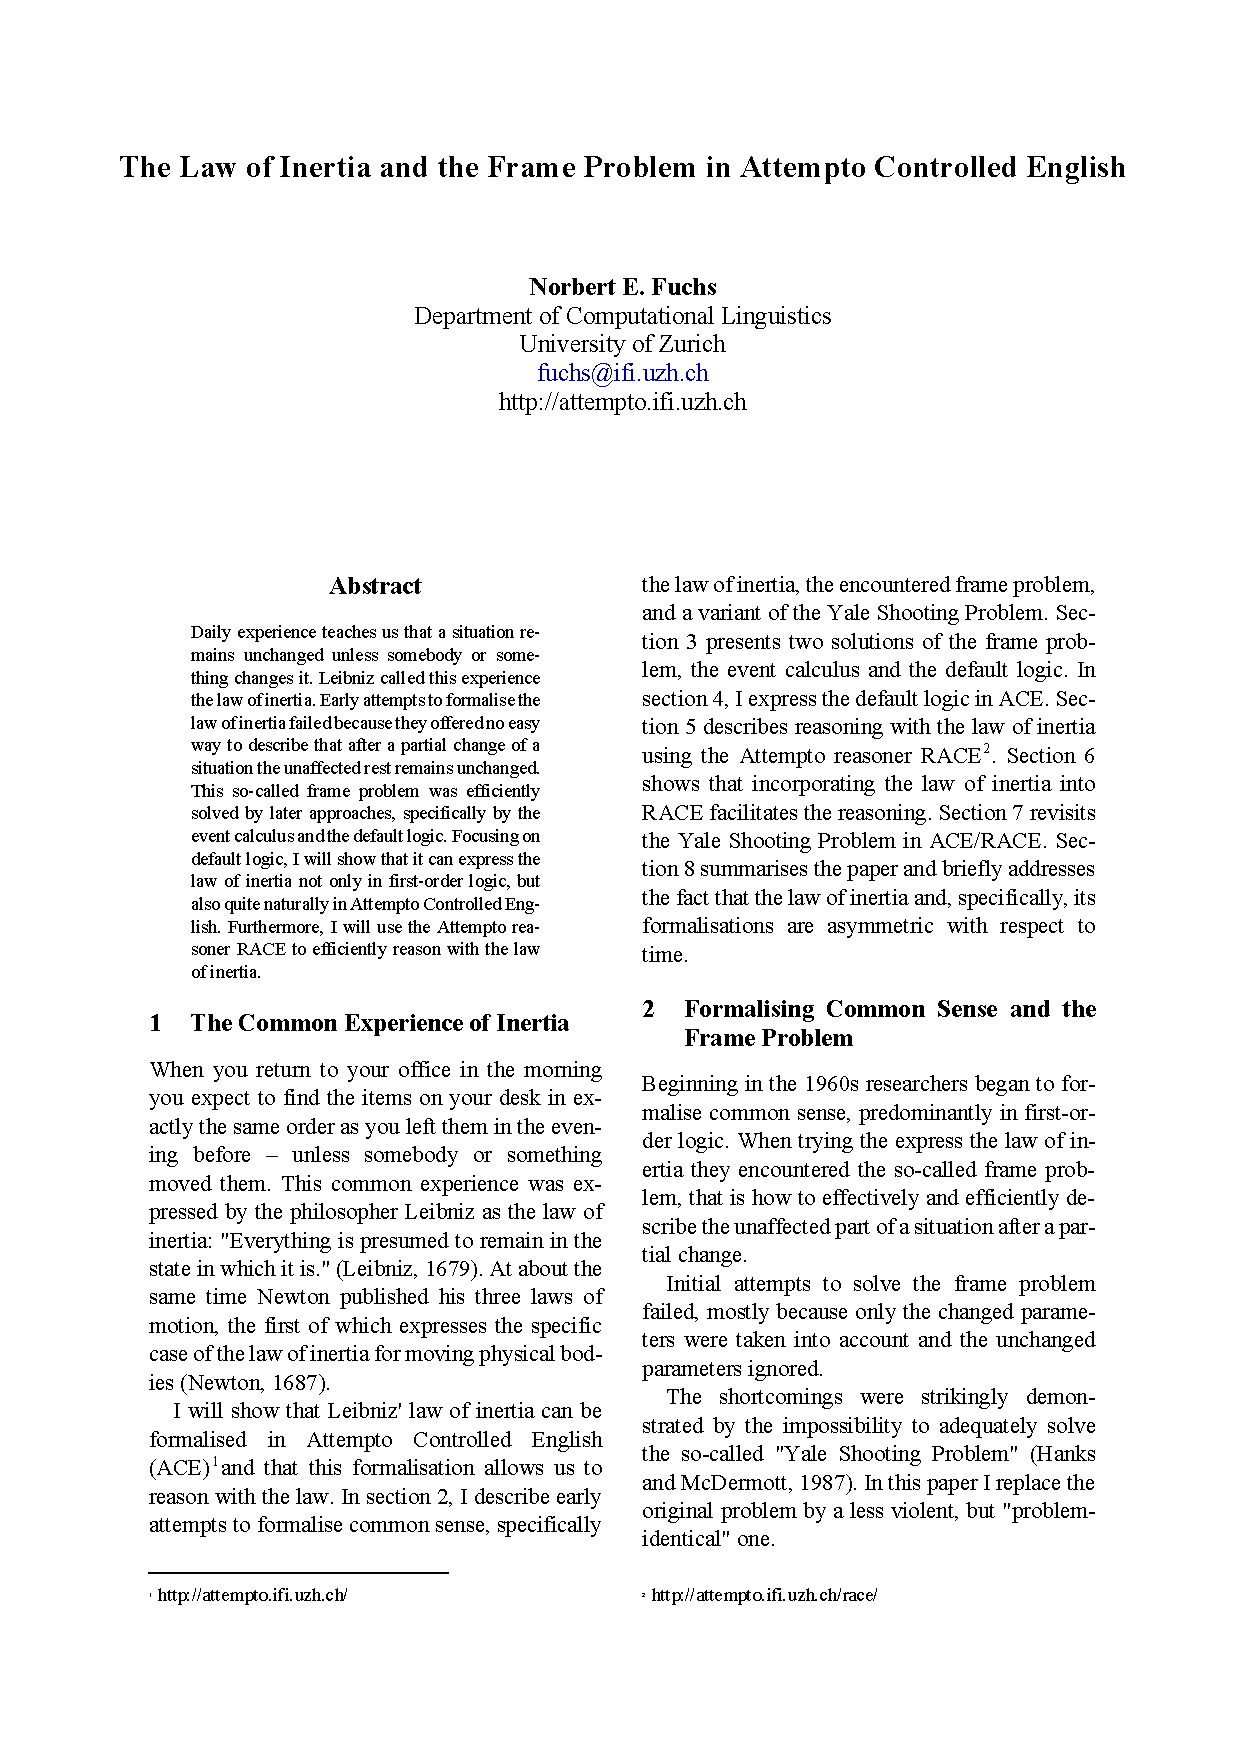
\includepdf[pages=-,pagecommand={}]{../cdrom/pdf/2021.cnl-1.7.pdf}

\invisiblesection{Norbert E. Fuchs. Reasoning in Attempto Controlled English: Mathematical and Functional Extensions}
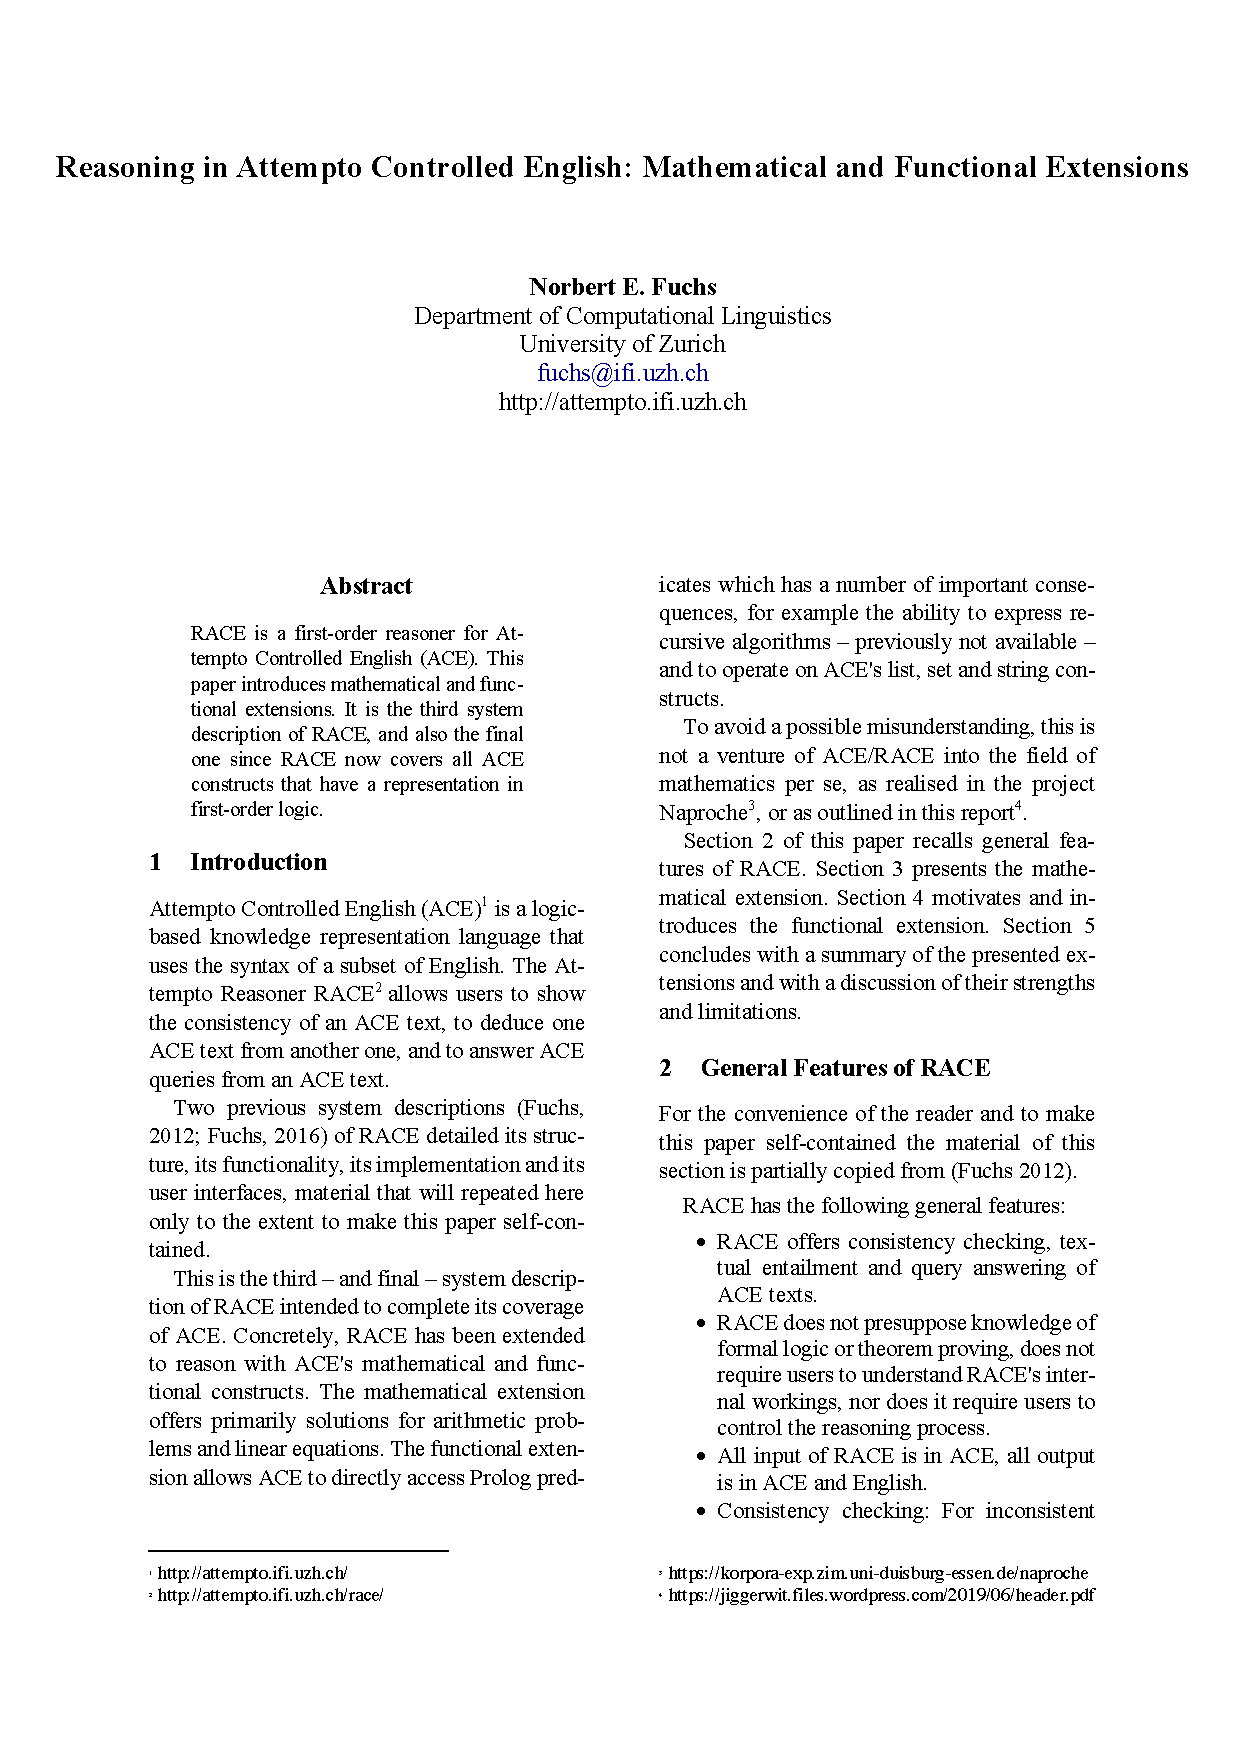
\includepdf[pages=-,pagecommand={}]{../cdrom/pdf/2021.cnl-1.8.pdf}

\invisiblesection{Ilona Wilmont, Diederik Dulfer, Jan Hof, Mischa Corsius and Stijn Hoppenbrouwers. A quality evaluation framework for a CNL for agile law execution}
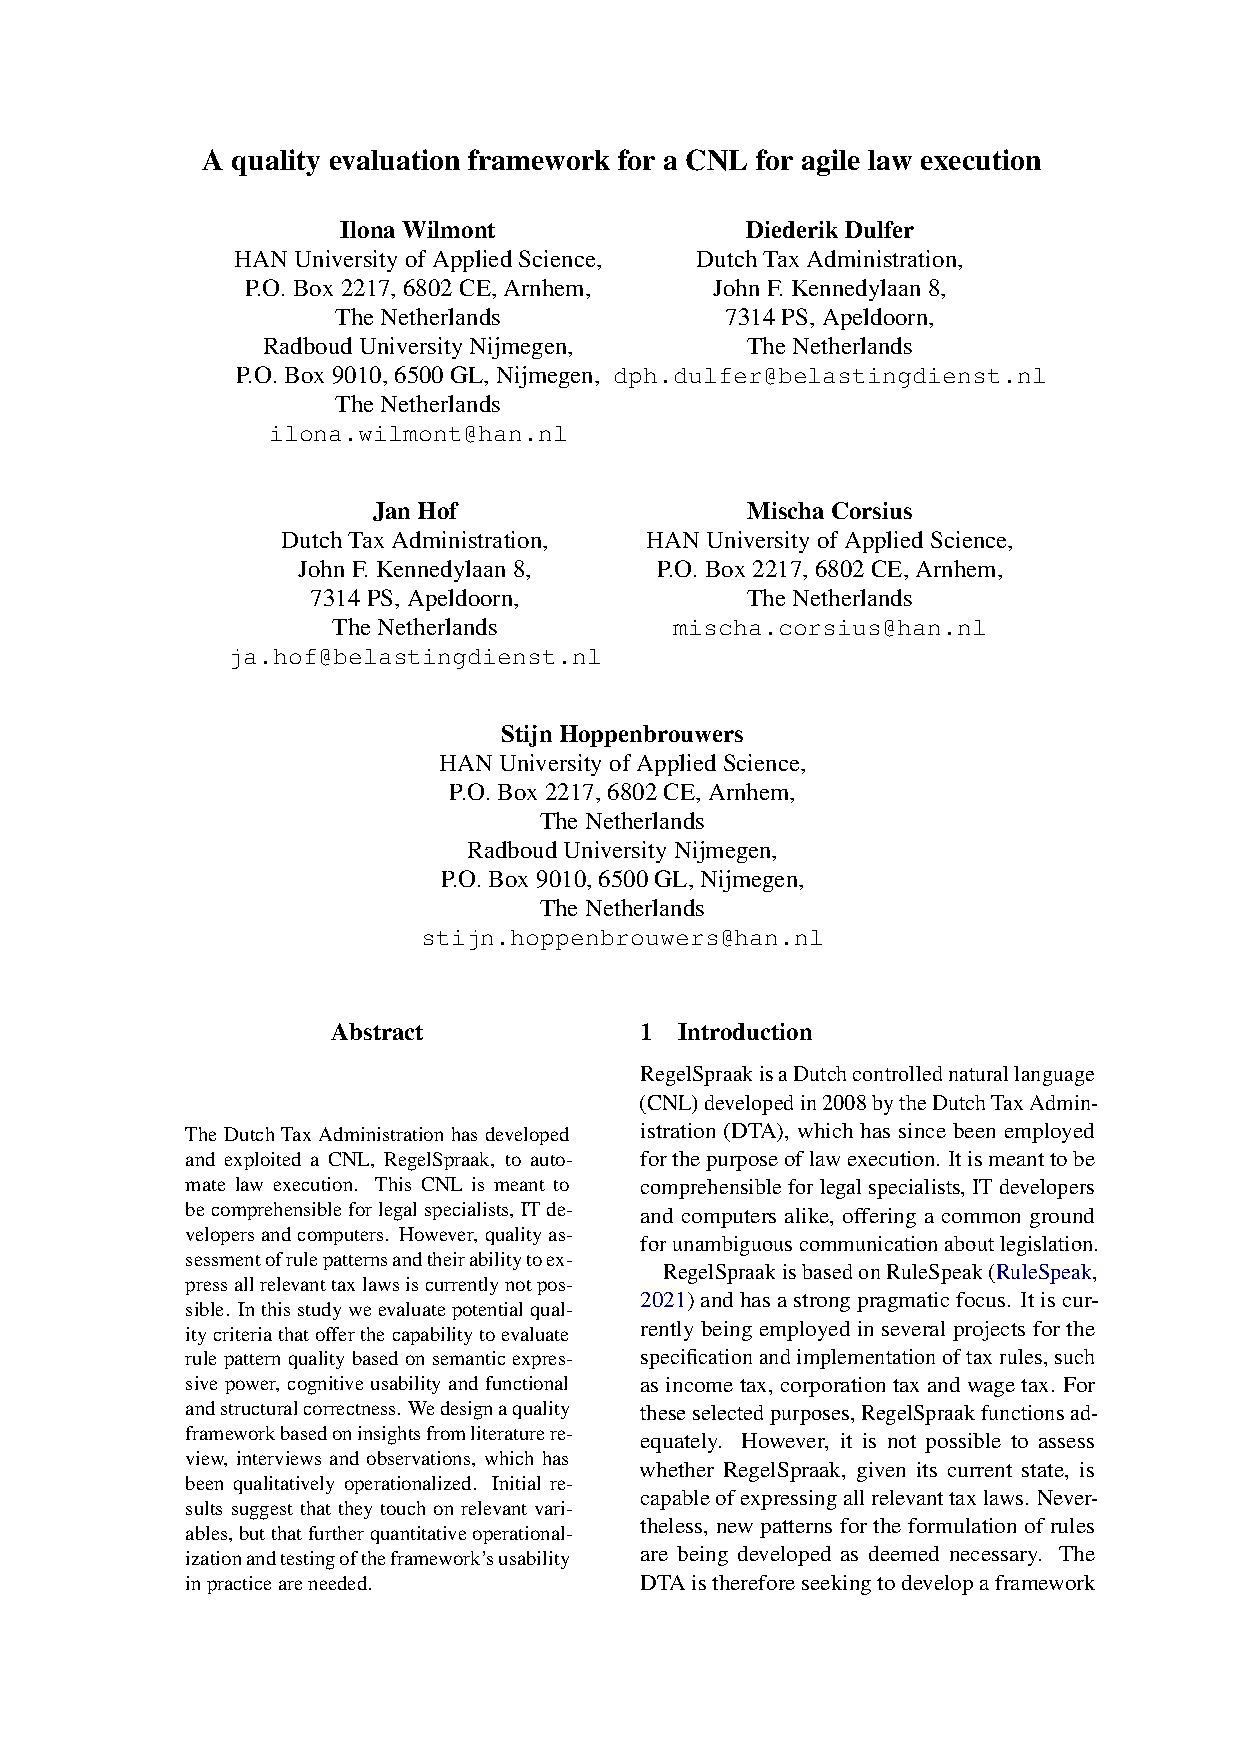
\includepdf[pages=-,pagecommand={}]{../cdrom/pdf/2021.cnl-1.9.pdf}

\invisiblesection{Inari Listenmaa, Maryam Hanafiah, Regina Cheong and Andreas Källberg. Towards CNL-based verbalization of computational contracts}
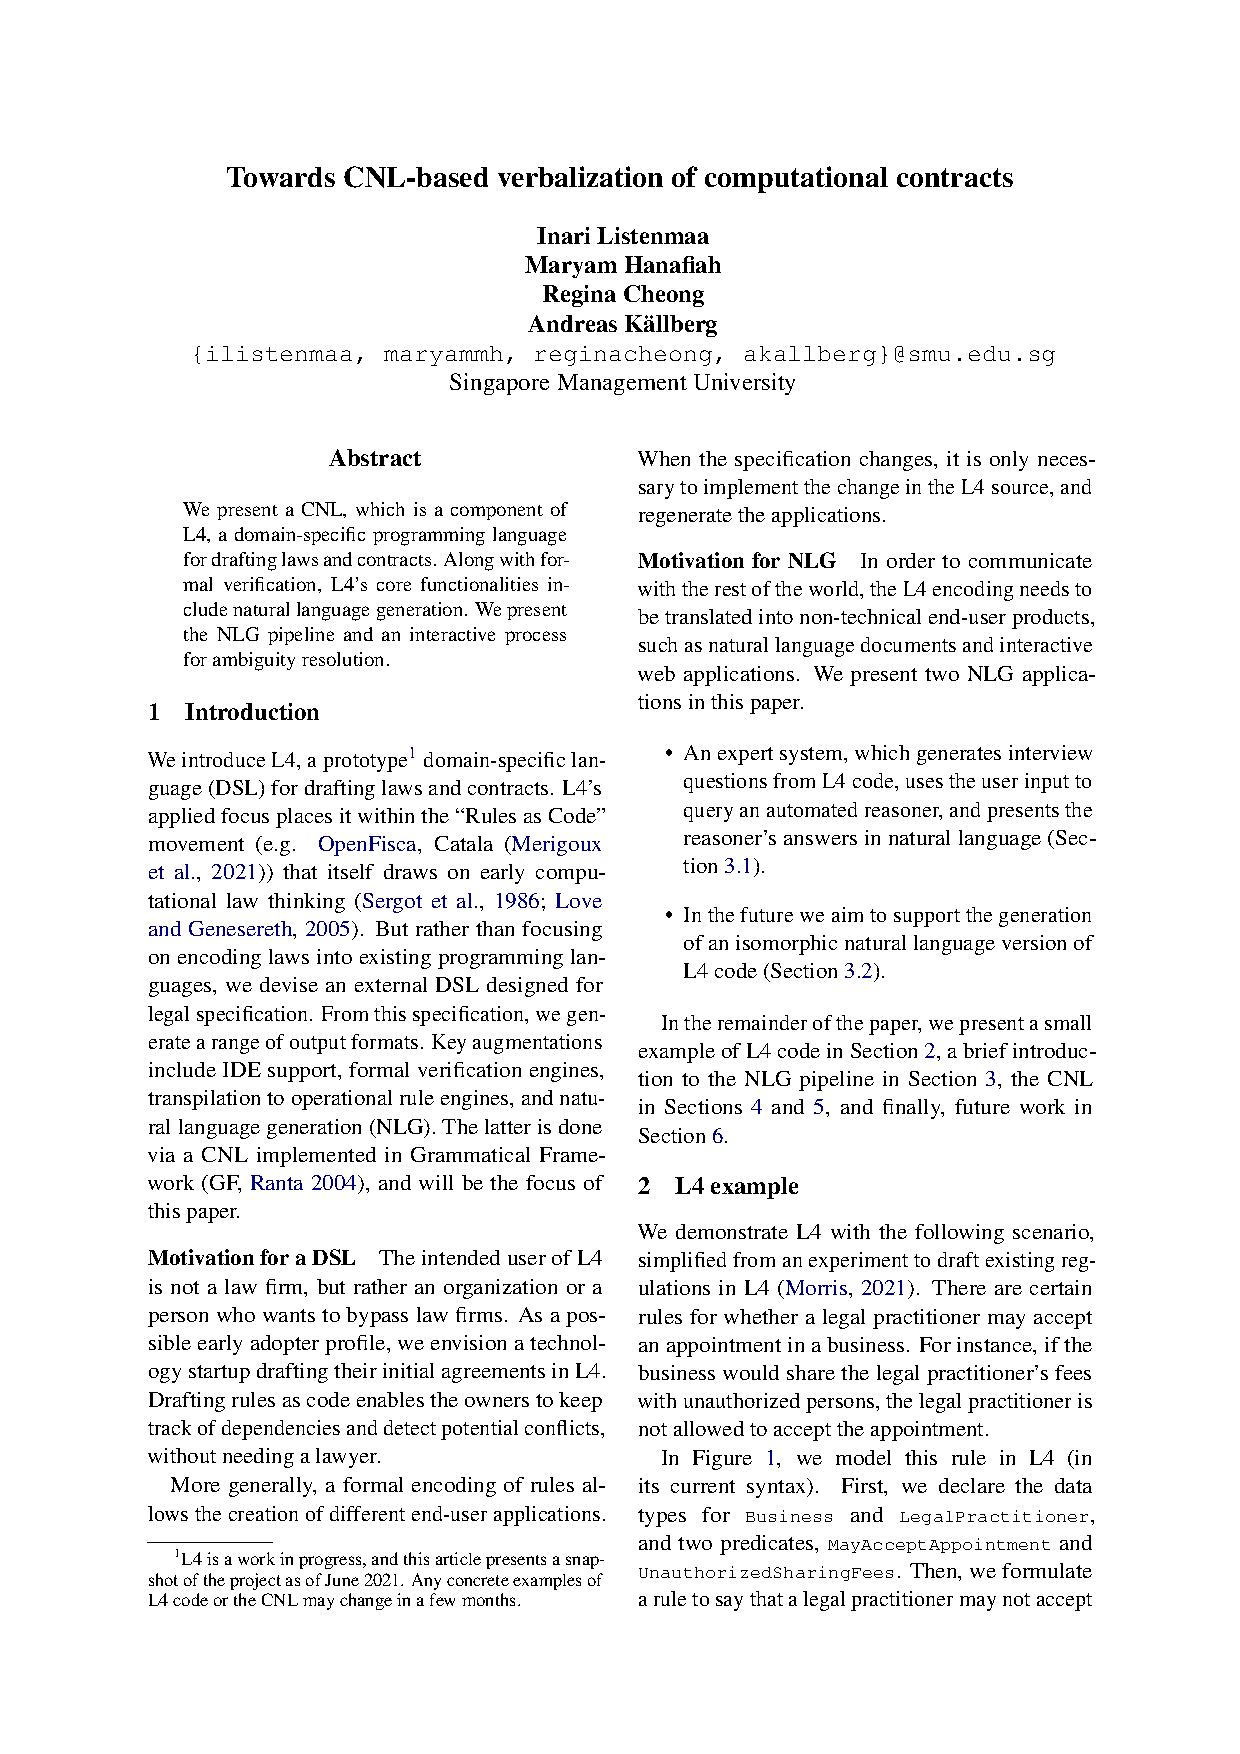
\includepdf[pages=-,pagecommand={}]{../cdrom/pdf/2021.cnl-1.10.pdf}

\invisiblesection{Mary-Jane Antia and C.Maria Keet. Assessing and Enhancing Bottom-up CNL Design for Competency Questions for Ontologies}
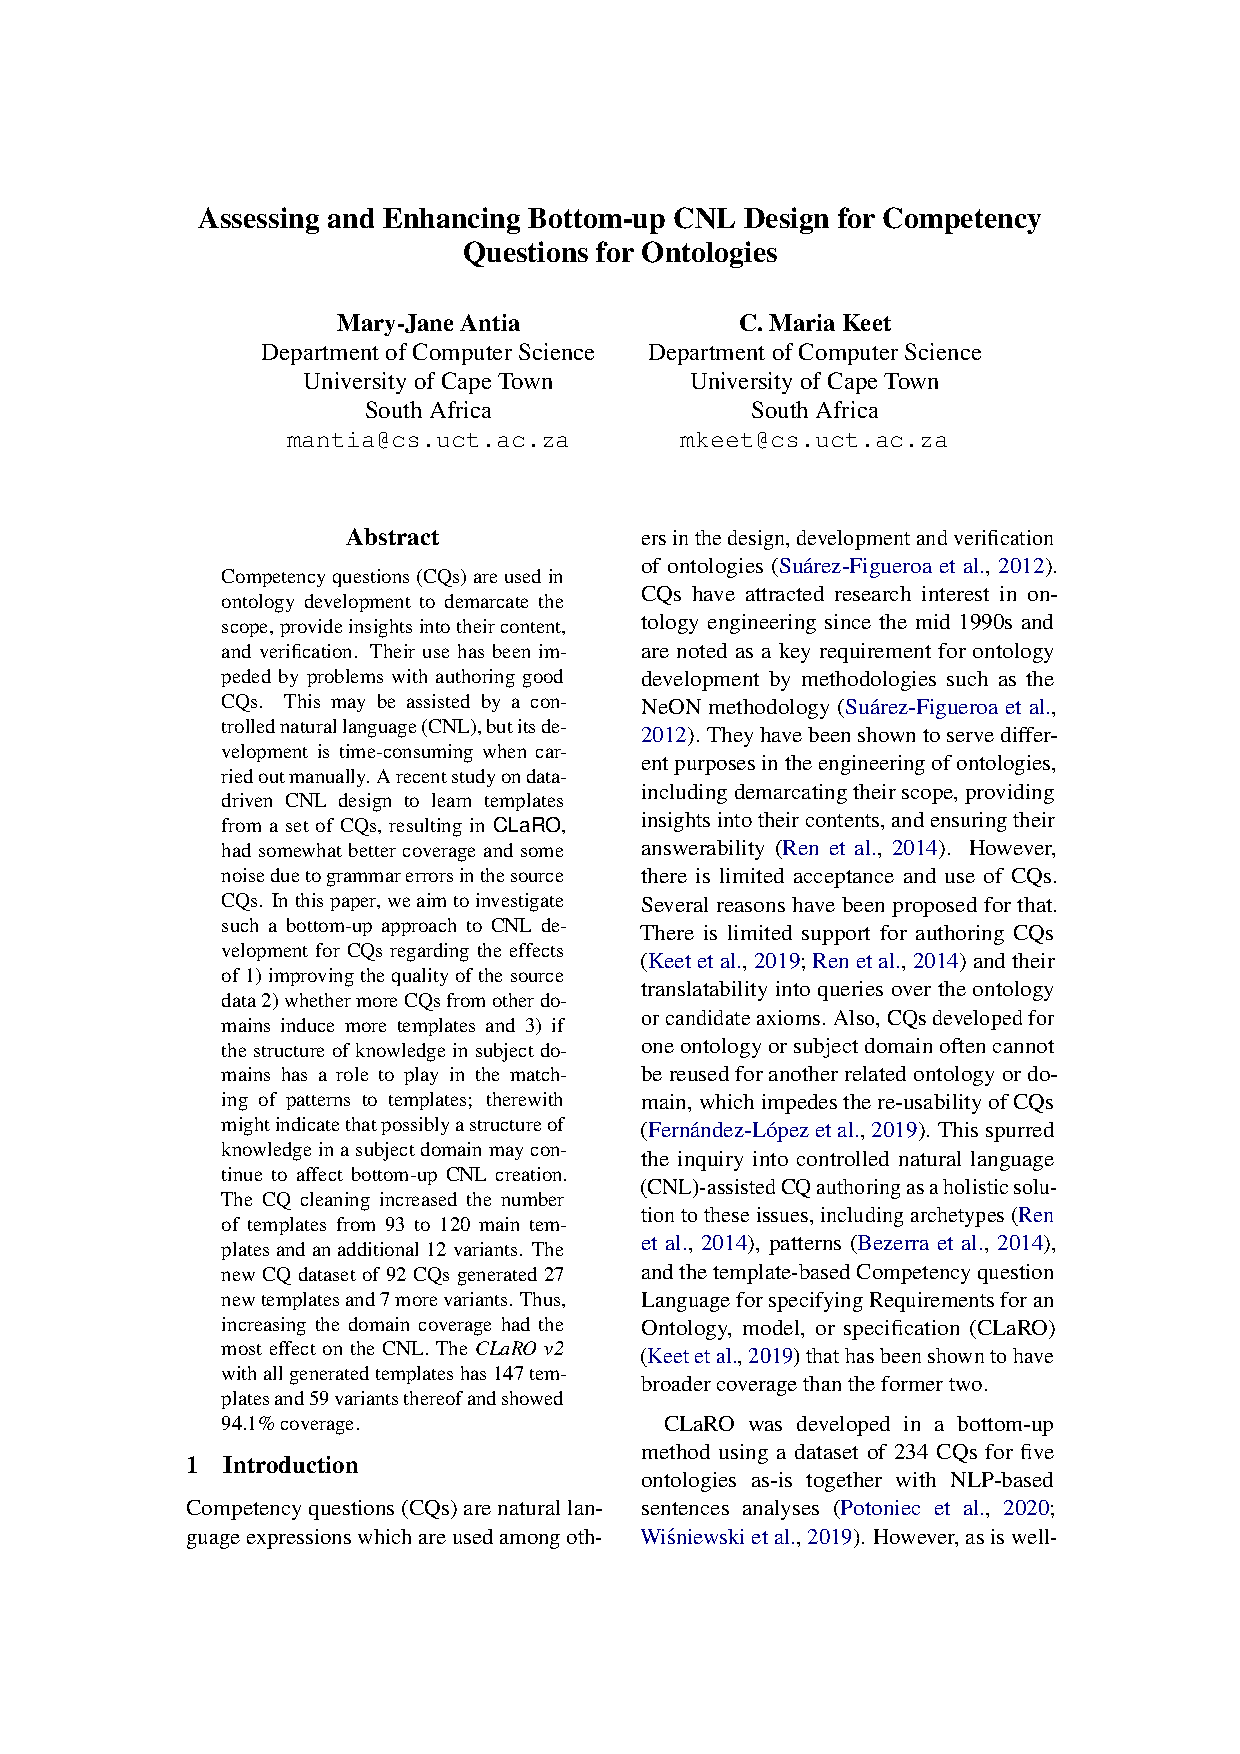
\includepdf[pages=-,pagecommand={}]{../cdrom/pdf/2021.cnl-1.11.pdf}


\refstepcounter{chapter}
\addcontentsline{toc}{chapter}{Short Papers}
\sectionmark{Short Papers}

\invisiblesection{Abdus Salam, Rolf Schwitter and Mehmet Orgun. Human-understandable and Machine-processable Explanations for Sub-symbolic Predictions}
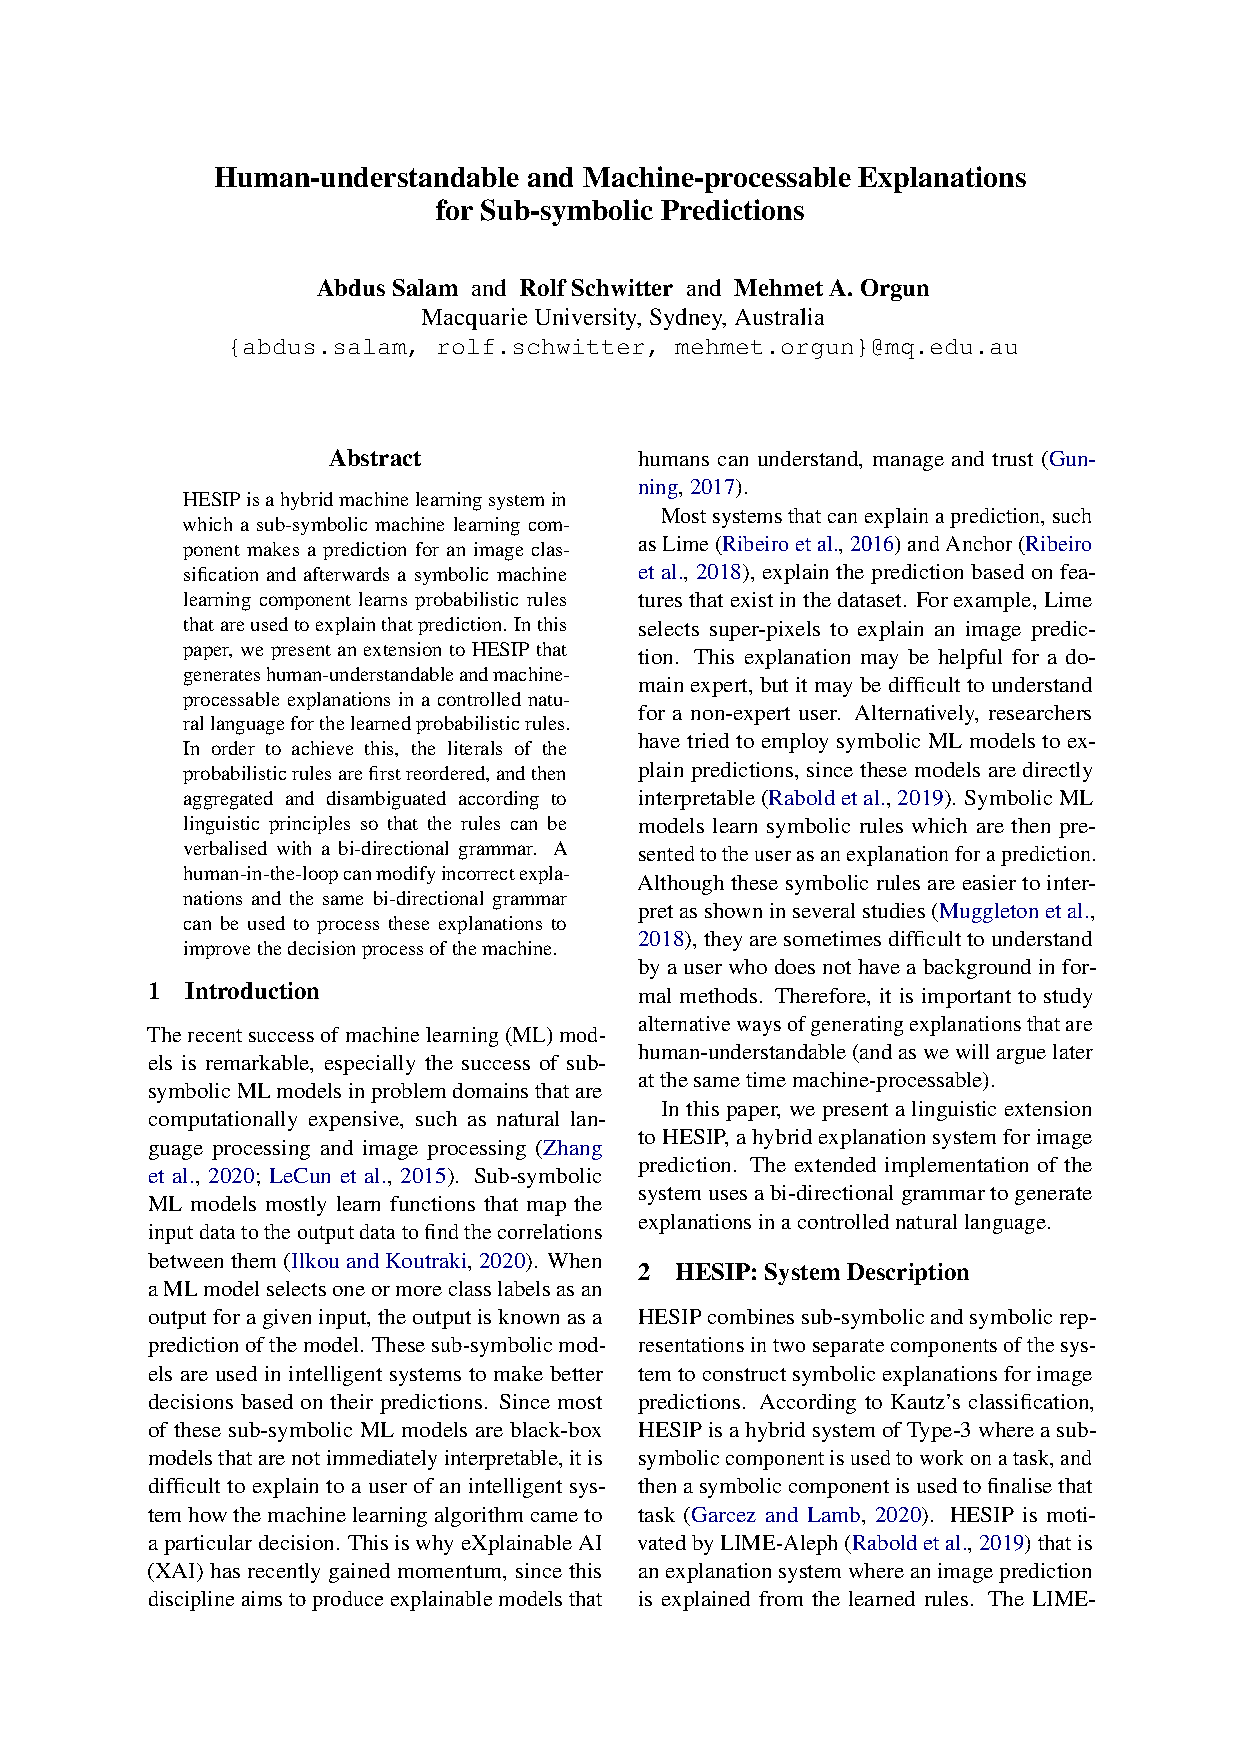
\includepdf[pages=-,pagecommand={}]{../cdrom/pdf/2021.cnl-1.12.pdf}

\invisiblesection{Lloyd Rutledge and Rudy Italiaander. Toward a Reference Architecture for Traceability in SBVR-based Systems}
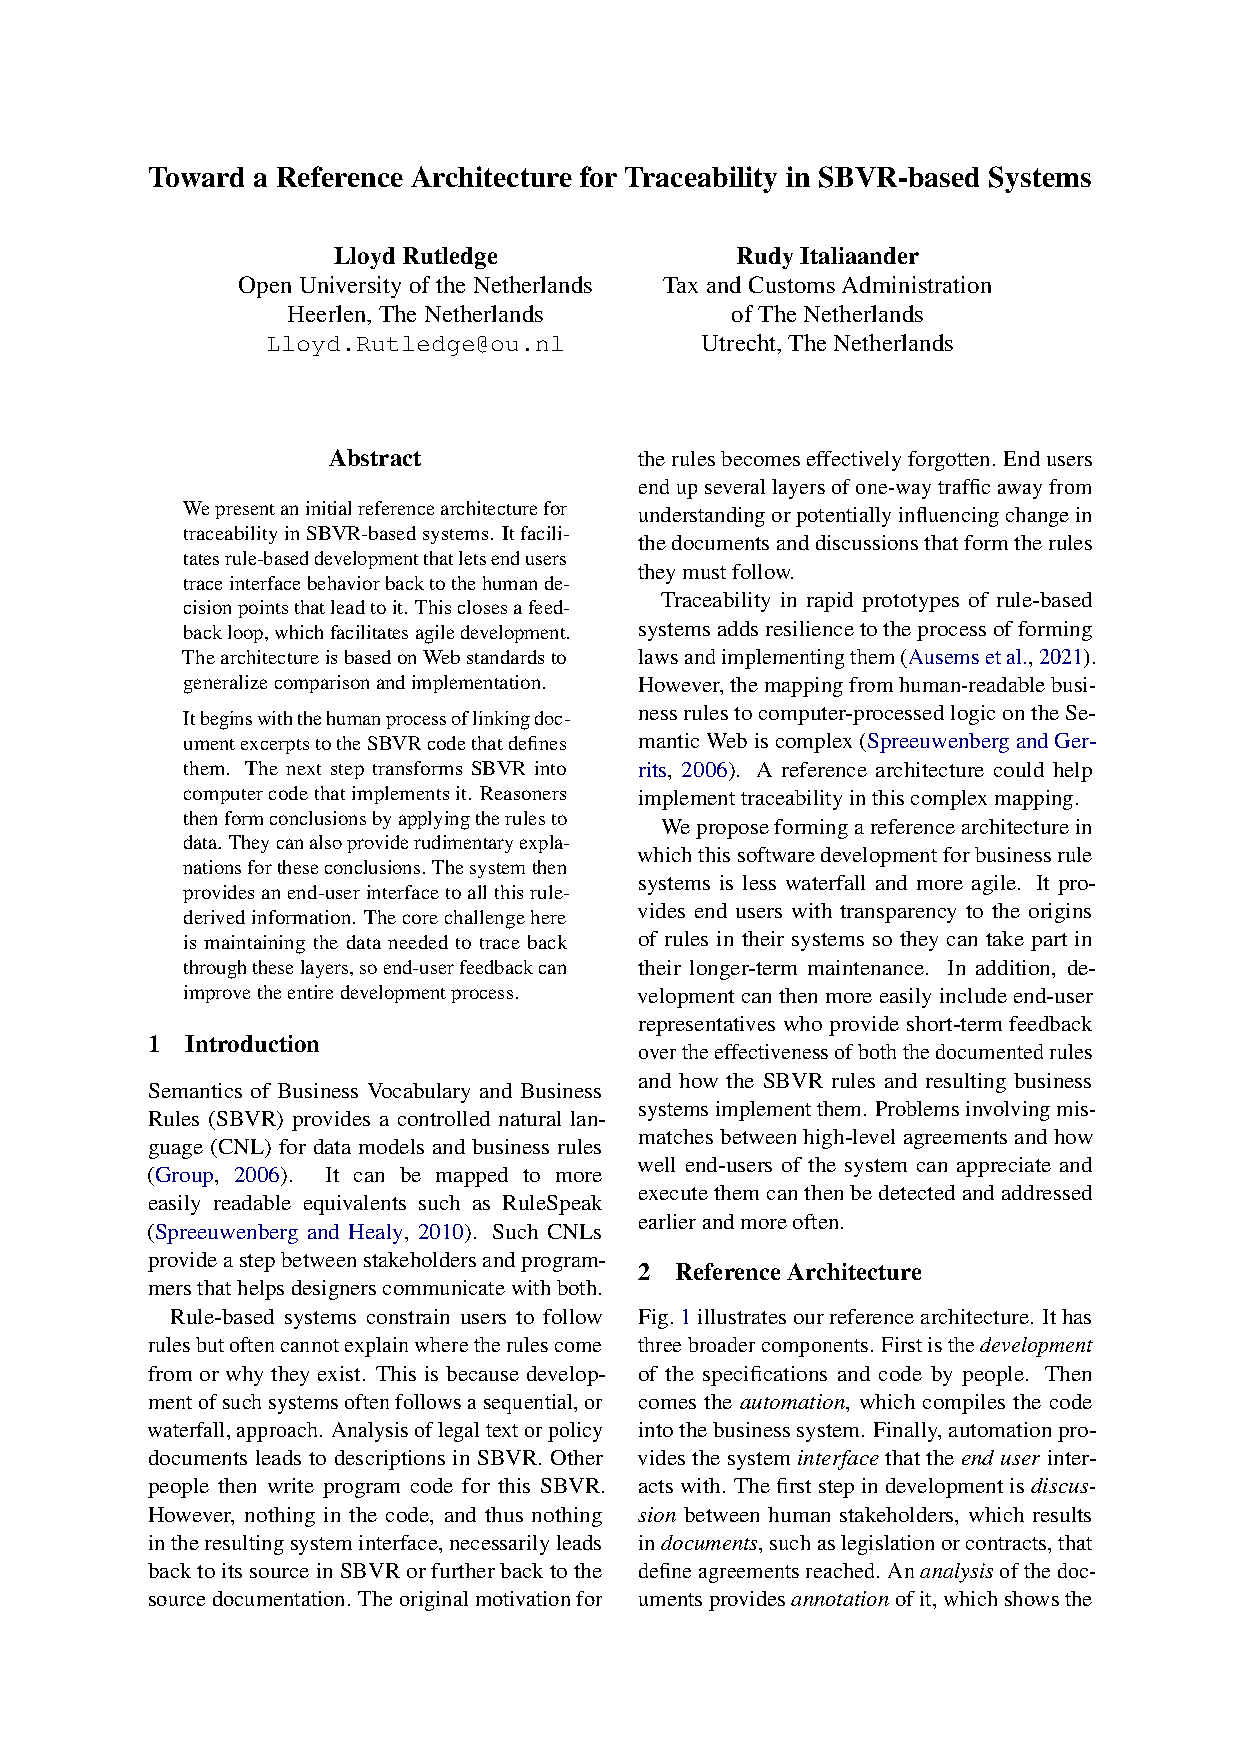
\includepdf[pages=-,pagecommand={}]{../cdrom/pdf/2021.cnl-1.13.pdf}

\invisiblesection{Joel Cedric Lengeling. Facilitating the application of Controlled Natural Language (CNL) to standardize communication in logistics and supply chain management}
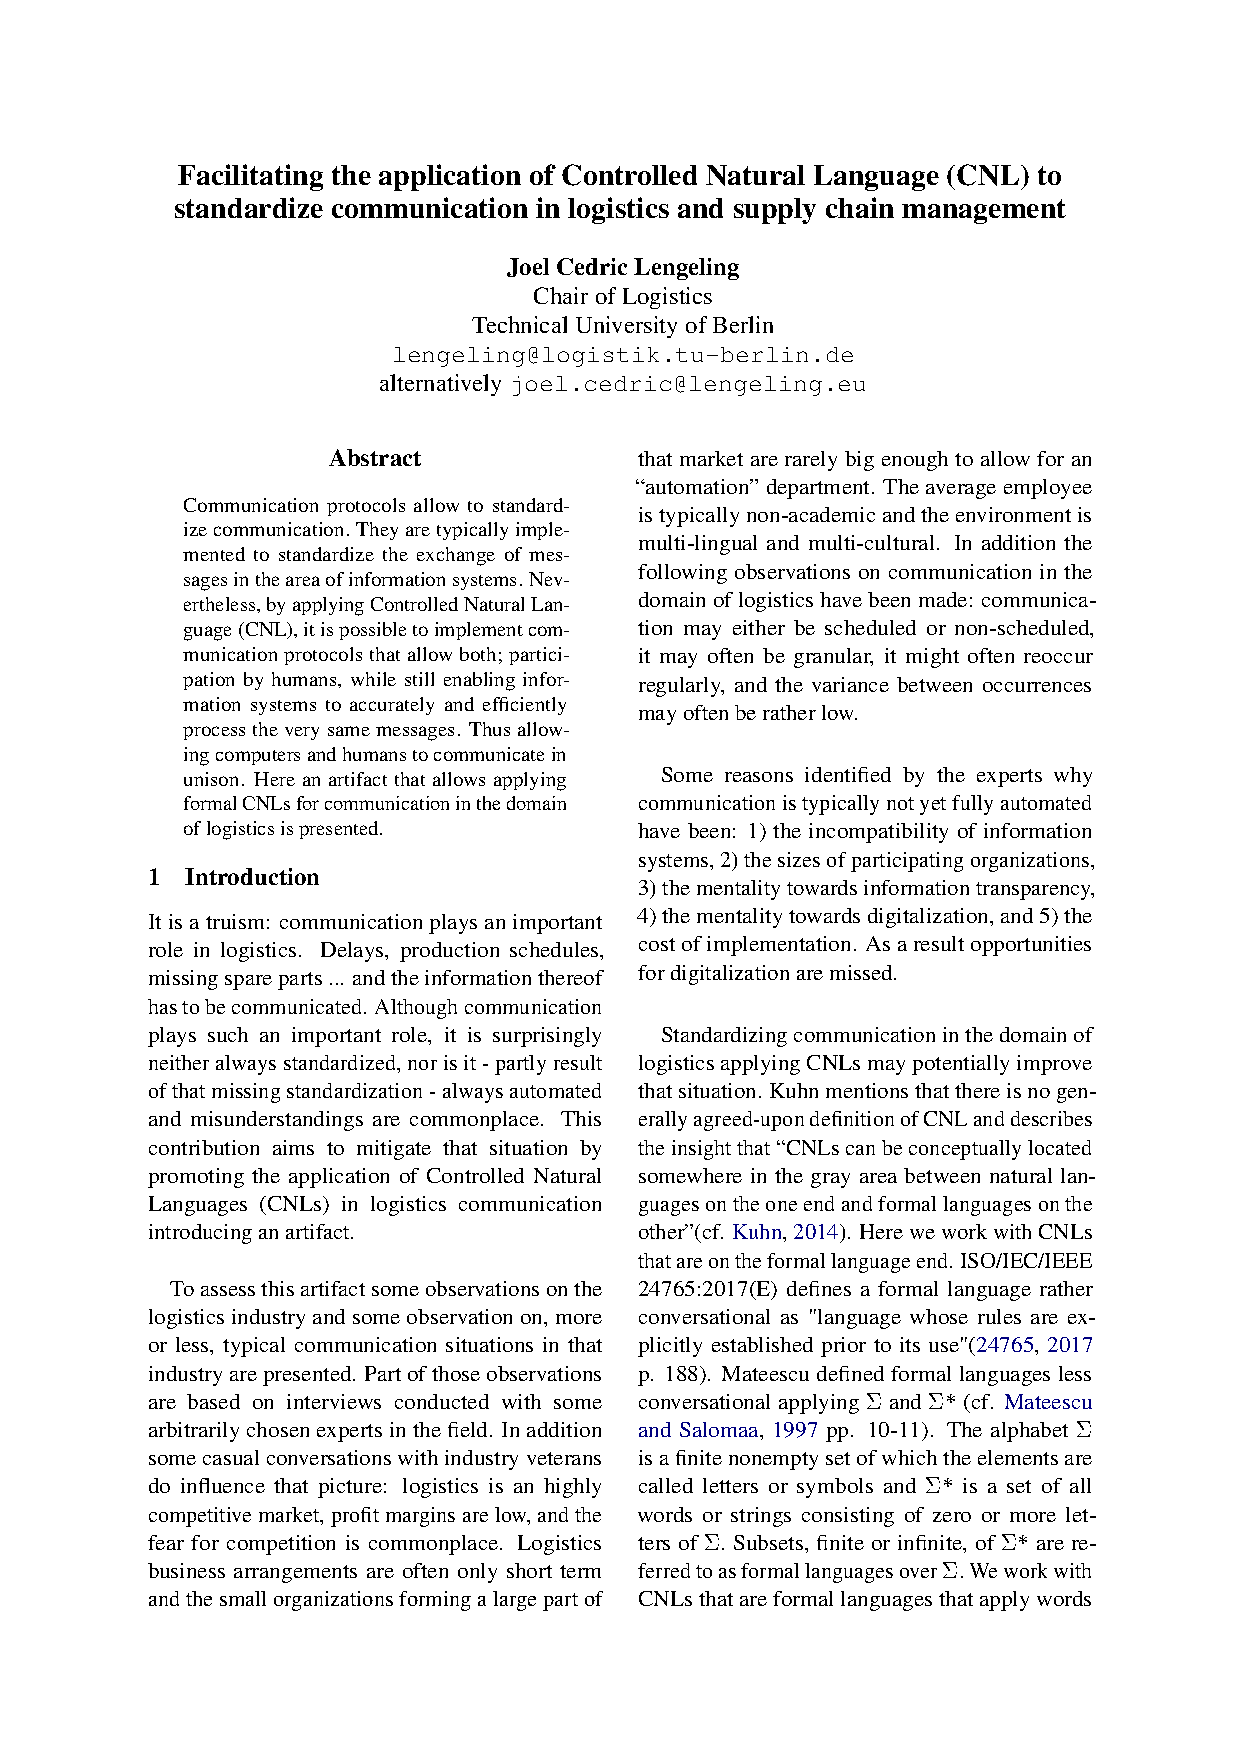
\includepdf[pages=-,pagecommand={}]{../cdrom/pdf/2021.cnl-1.14.pdf}

\invisiblesection{Joan Byamugisha and Nomonde Khalo. A CNL-based Method for Detecting Disease Negation}
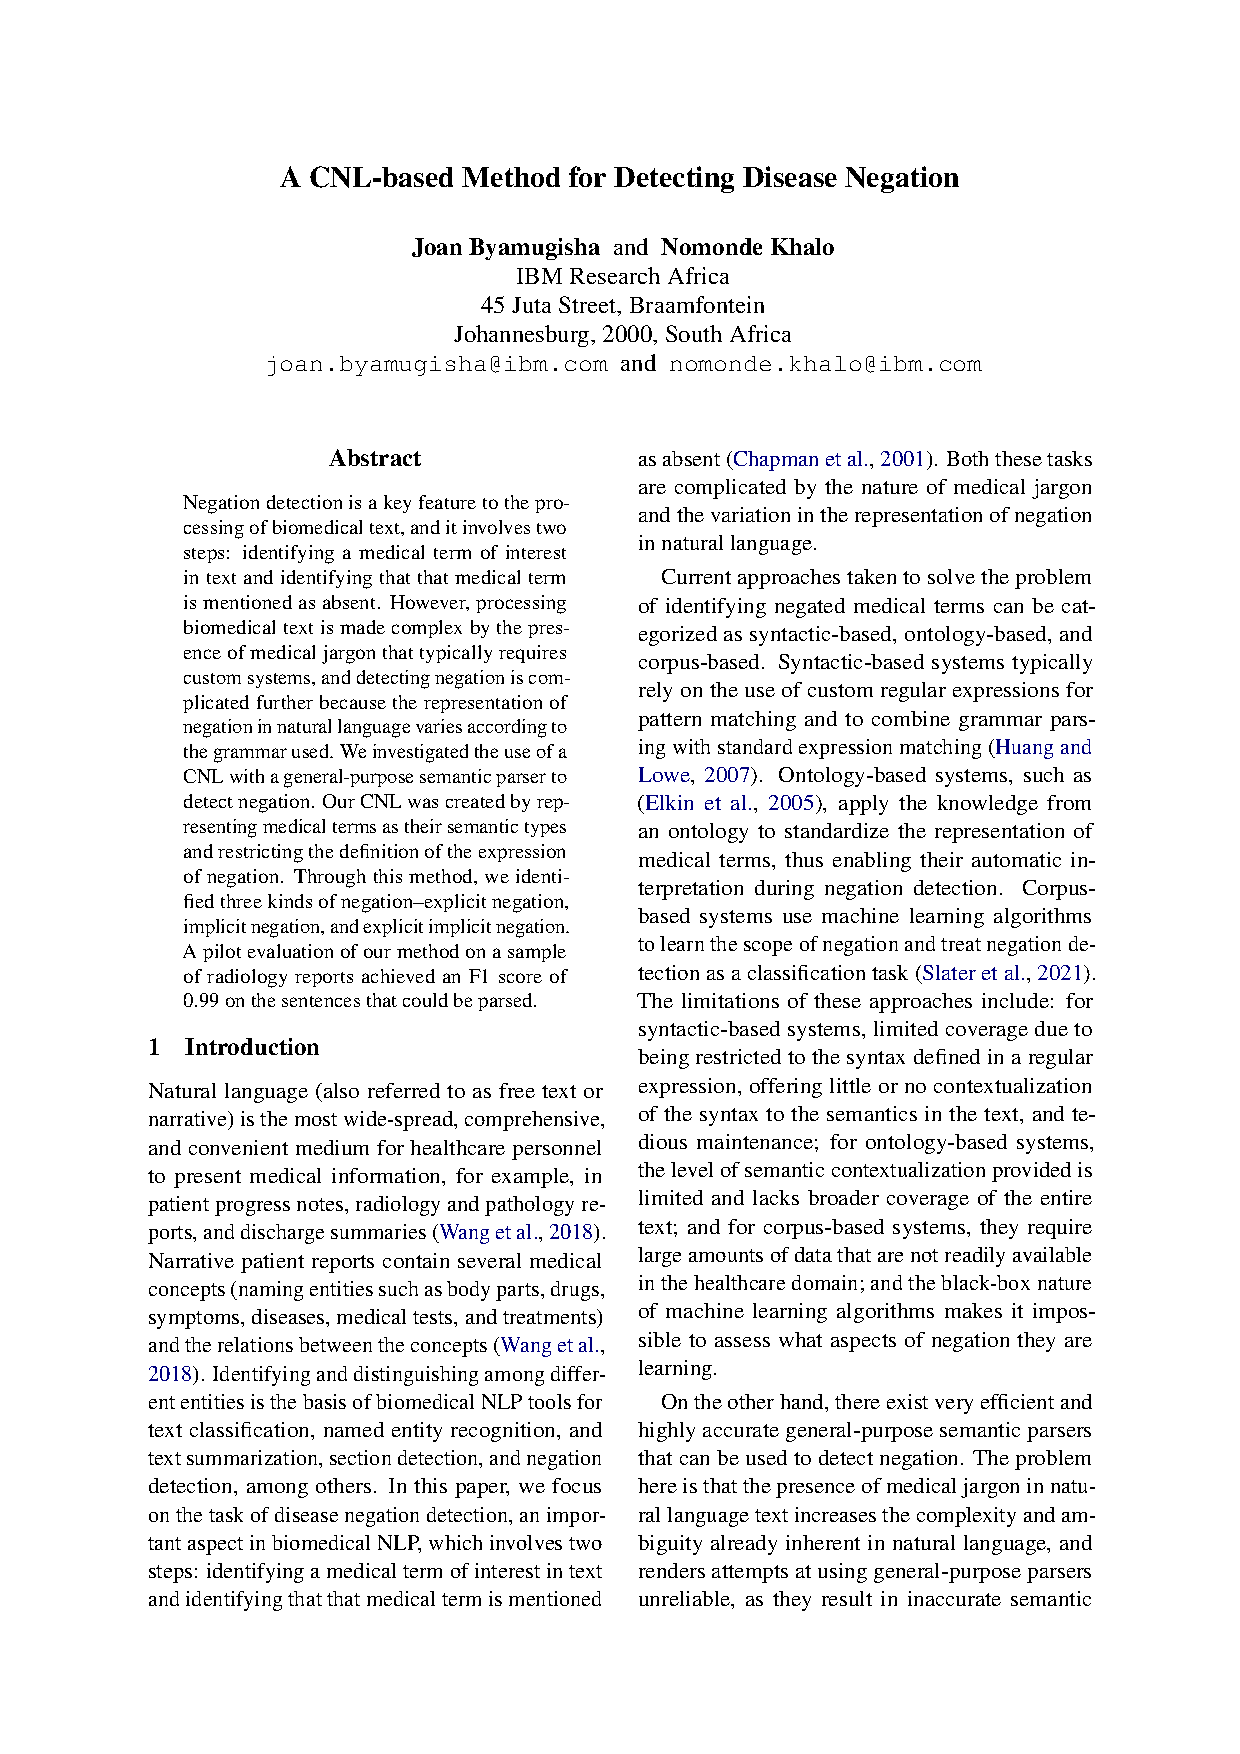
\includepdf[pages=-,pagecommand={}]{../cdrom/pdf/2021.cnl-1.15.pdf}

\invisiblesection{Michael Hsiao. Multi-Phase Context Vectors for Generating Feedback for Natural-Language Based Programming}
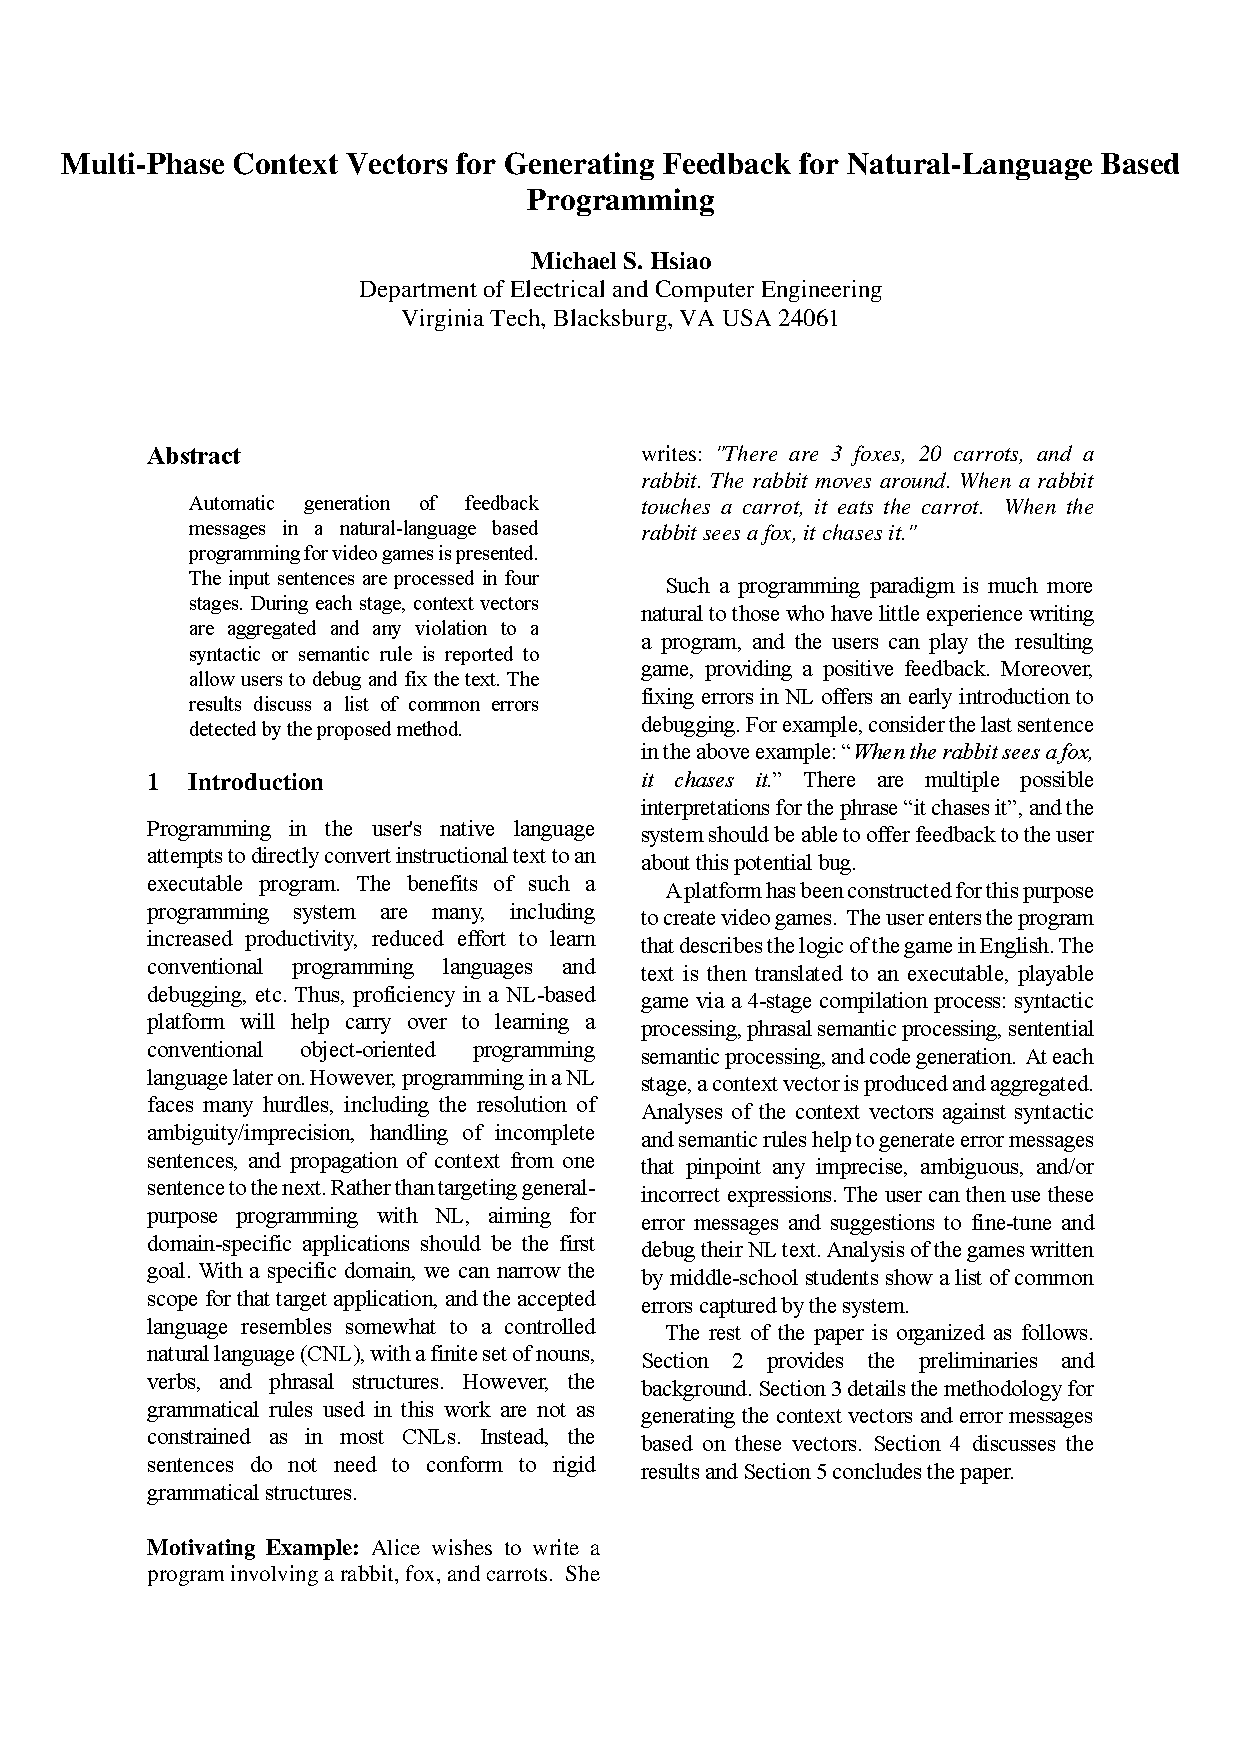
\includepdf[pages=-,pagecommand={}]{../cdrom/pdf/2021.cnl-1.16.pdf}



